% Created 2021-02-07 Sun 10:40
% Intended LaTeX compiler: pdflatex
\documentclass[11pt]{article}
\usepackage[utf8]{inputenc}
\usepackage[T1]{fontenc}
\usepackage{graphicx}
\usepackage{grffile}
\usepackage{longtable}
\usepackage{wrapfig}
\usepackage{rotating}
\usepackage[normalem]{ulem}
\usepackage{amsmath}
\usepackage{textcomp}
\usepackage{amssymb}
\usepackage{capt-of}
\usepackage{hyperref}
\author{Francesco Codice' }
\date{\today}
\title{}
\hypersetup{
 pdfauthor={Francesco Codice' },
 pdftitle={},
 pdfkeywords={},
 pdfsubject={},
 pdfcreator={Emacs 27.1.90 (Org mode 9.5)}, 
 pdflang={English}}
\begin{document}

\tableofcontents

\section{Introduction}
\label{sec:orgd03cc9a}

\textbf{Information flow}
\begin{center}
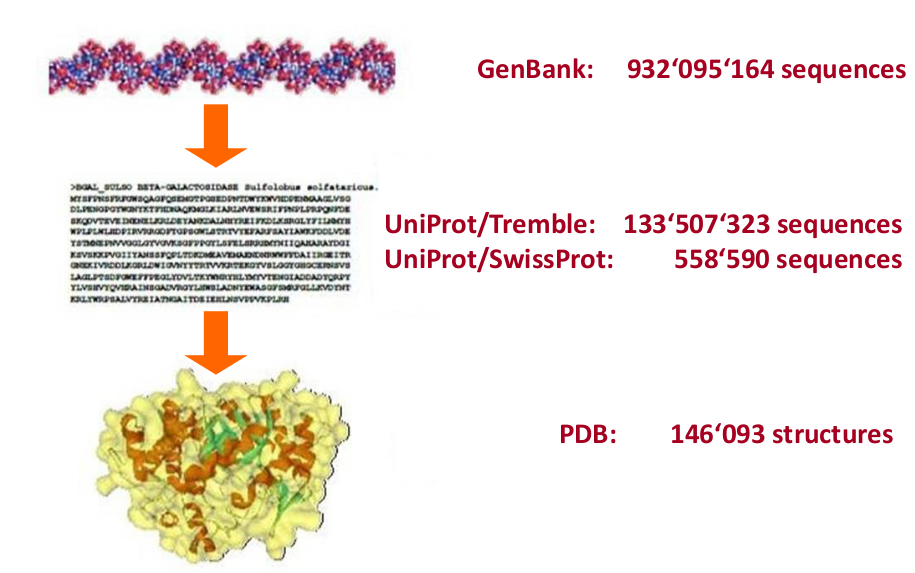
\includegraphics[width=.9\linewidth]{imgs/Introduction/2021-01-31_17-31-08_screenshot.png}
\end{center}



\textbf{Type of data} : 
\begin{itemize}
\item \textbf{Primary data} (experimental results):
\begin{itemize}
\item Genomes
\item Protein Sequences
\item Protein Structures Interactions
\end{itemize}
\item \textbf{Secondary data} (derived info)
\begin{itemize}
\item Protein folds
\item Protein families
\item Genome comparisations
\end{itemize}
\end{itemize}



\textbf{Annotation/Curation} :
\begin{itemize}
\item \textbf{Raw Data} : Protein sequence only
\item \textbf{Annotated Data} : Protein sequence with function, localization, expression info, links etc.
The annotation can be : \emph{Manual} or \emph{Automatic}
\end{itemize}


\textbf{Common problems} : 
\begin{itemize}
\item Quality check : if error enter a database they tend to propagate into other databases
they are difficult to estirpate.
\item Lack of standardization : lack of schema and lack of common nomenclature
\item Integration : is important to integrate more databases. By fusion(uniprot) or by links.
\end{itemize}

\textbf{Main Bioinformatics databases}\\
\begin{itemize}
\item Uniprot: A comprehensive resource for protein sequence and functional annotation.
\item Ensembl: Genome browser, API and database, providing access to reference genome annotation
\item PDBe: The European resource for the collection, organisation and dissemination
of 3D structural data (from PDB).
\item InterPro : A databse for the classification of proteins into families, domains
and conserved sites.
\end{itemize}

\subsection{Database introduction}
\label{sec:org202a1a5}
A database is a large structured set of persistent data, usually in
computer-readable form

\textbf{Database terminology}
\begin{itemize}
\item \emph{Table} : A collection of closely related columns. A table consists of rows each of which shares the same columns but vary in the column values.
\item \emph{Record} : A record is a collection of fields, possibly of different data
types, typically in a fixed number and sequence
\item \emph{Key} : A Key is a data item that exclusively identifies a record. In other
words, key is a set of column(s) that is used to uniquely identify the record
in a table
\end{itemize}

\textbf{DBMS}\\
DBMS software primarily functions as an interface between the end user and the
database, simultaneously managing the data, the database engine, and the
database schema in order to facilitate the organization and manipulation of data
Allows the user to:
\begin{itemize}
\item Access data
\item Manipulate data
\item Preserve the integrity
\item Deal with security
\end{itemize}

\textbf{DBMS Models}:
\begin{itemize}
\item Flat file
\item Hierical Models
\item Relational Model
\item Object-Oriented Model
\end{itemize}


\subsection{Relational Model}
\label{sec:orgfde49fd}
\begin{itemize}
\item Schema : logical structure of the data. \emph{Intensional} part
\item Instance : is the set of actual data. \emph{Extensional} part
\end{itemize}


\textbf{How to store a Schema}\\
\begin{itemize}
\item Flat file – simple and available to all
\item XML – eXtensible Markup Language (Markups instruct the software displaying the
text)
\item ASN.1 – Abstract Syntax Notation One (NCBI uses ASN.1 for data storage and
retrieval)
\end{itemize}



\section{Pubmed}
\label{sec:orgee5d967}
The National Center for Biotechnology Information (NCBI)(\textsubscript{www.ncbi.nlm.nih.gov}\_)
Created in 1988 as a part of the National Library of Medicine (NLM) at the
National Institute of Health (NIH).


\textbf{PubMed sections}\\
\begin{itemize}
\item PubMed free Medline
\item PubMed Central : full text online access
\item MeSH database (Medial Subject Headings) : controlled vocabulary thesaurus
\end{itemize}


\textbf{Why databases search is important?}\\
\begin{itemize}
\item The scientific literature increases by 2000 pages every minute.
\item It would take 5 years to read the new scientific literature produced in 1 day.
\end{itemize}
\(\rightarrow\) Search engines play an essential role for picking out the right articles



\subsection{Quering}
\label{sec:org757a758}
\textbf{How to search?}\\
\begin{itemize}
\item \textbf{by Author} : name and initials with ['author'] tag (e.g. 'lesk am')
\item \textbf{by Subject} : put the keyboard in search field ('e.g. 'evolution')
\item \textbf{by Journal} : put the name of the journal with ['journal'] tag
\end{itemize}

PubMed uses \textbf{Automatic Term Mapping} : for any terms entered without a qualifier are looked
up against the following translation tables and indexes in a distinct order
\begin{enumerate}
\item MeSH Translation Table (terms like diseases, phenomena etc.)
\item Journal Translation Table
\item Author Index
\end{enumerate}

It performs a translation and build the database query automatically

\uline{Example}
Search: lesk am evolution
\begin{verbatim}
lesk am[Author] AND ("biological evolution"[MeSH Terms] OR ("biological"[All Fields] 
AND "evolution"[All Fields]) OR "biological evolution"[All Fields] OR "evolution"[All Fields]
OR "evolution s"[All Fields] OR "evolutional"[All Fields] OR "evolutions"[All Fields] 
OR "evolutive"[All Fields] OR "evolutivity"[All Fields])
\end{verbatim}


For any database we usually have table that list all the possible \emph{search fields}
\begin{figure}[htbp]
\centering
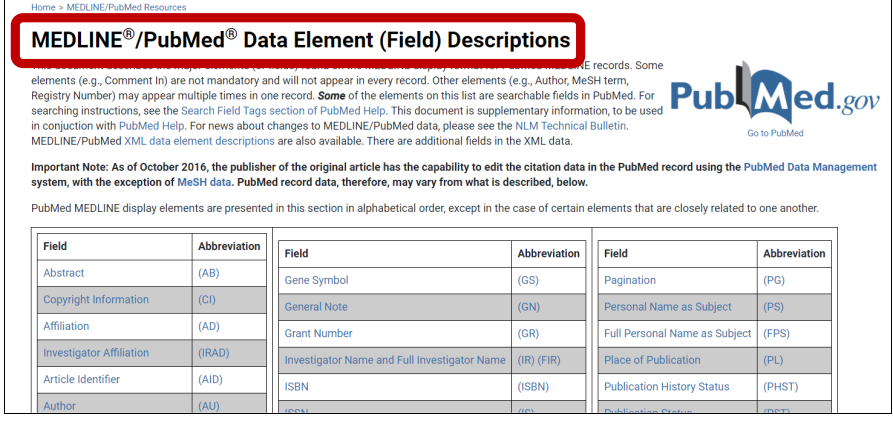
\includegraphics[width=.9\linewidth]{Introduction/field_Description_2020-11-17_14-42-00.png}
\caption{Field Description Page of PubMed}
\end{figure}

\subsubsection{MeSH}
\label{sec:org03a15f0}
MeSH vocabulary is divided into four types of terms. The main ones are the
``headings'' (also known as MeSH headings or descriptors[2]), which describe the
subject of each article (e.g., ``Body Weight'', ``Brain Edema'' or ``Critical Care
Nursing'').

\begin{itemize}
\item Search MeSH db with a keyword
\item click on the MeSH term, look at “Related information`` and search in Pubmed
\item for restricting use ``Major Topics''
\end{itemize}


\subsubsection{Api access}
\label{sec:org41c1f18}
Entrez Direct (EDirect) provides access to the NCBI's suite of interconnected databases
(pubblications, sequences, structues, genes, variations, expressions, etc.) from a 
UNIX terminal windows.

\textbf{Entrez Dirext Functions}\\
\begin{itemize}
\item \textbf{esearch} : performs a new Entrex search using terms in indexed fields
\item \textbf{efetch} : downloads records or reports in a designated format
\item \textbf{xtract} : converts EDirect XML output into a table of data values
\item \textbf{epost} : uploads unique indentifiers (UIDs) or sequence accession numbers
\end{itemize}


\subsection{Exercises}
\label{sec:orgdaf7bfb}
\subsubsection{Exercise 1}
\label{sec:org92ff3a2}
\begin{itemize}
\item \textbf{Question} : Within PubMed, search for articles which contain as ``Text Word''
``circadian rhythms'' and either ``cortisol'' or ``melatonin''. Limit your search to
articles which contain ``humans'' as a MeSH term, and exclude all Review
articles. How many entries have you found?
\item \textbf{Answer}
953 entries are present for this query.
The query used is the following
\begin{verbatim}
    "circadian rhythms "[Text Word] AND (melatonin[Text Word] OR cortisol[Text Word]) AND "Humans"[MeSH Terms] NOT "review"[Publication Type]
\end{verbatim}
\end{itemize}

\subsubsection{Exercise 2}
\label{sec:orgf532c20}
\begin{itemize}
\item \textbf{Question} : Find all articles with first or last author “Smith”, which have
been ``nih funded'' (hint: check in ``Filter''), whose major topics is “Alzheimer
disease”, dealing in particular with the diagnosis of such disease. How many
articles have you found ?

\item \textbf{Answer}

\begin{verbatim}
    ((Smith[Author - Last] OR Smith[Author - First]) AND "nih funded"[Filter] AND "Alzheimer disease/Diagnosis"[MeSH Major Topic])
\end{verbatim}
\end{itemize}

\section{UniProt}
\label{sec:org8256e66}
A comprehensive resource for protein sequence and functional annotation.

It is a consortium
\begin{itemize}
\item \textbf{SIB} (Swiss Institute of Bioinformatics) : /UniProtKB/(UniProt Knowledgebase) \uline{\emph{Swiss-Prot}}
\item \textbf{EBI} (European Bioinformatics Institute) : UniProtKB// \uline{\emph{TrEMBL}} and \uline{\emph{UniParc}} (UniProt Archive)
\item \textbf{PIR} (Protein Information Resource) : \uline{\emph{UniRef}} (UniProt Reference Cluter)
\end{itemize}


\textbf{UniProt Data Flow}
EMBL(Cds) \(\rightarrow_{\text{(Translation)(Automatic Annotation)}}\)  \(\rightarrow\) TrEMBL(Protein) \(\rightarrow_{\text{(Manual Curation)}}\) Swiss-Prot(Protein)

\begin{figure}[htbp]
\centering
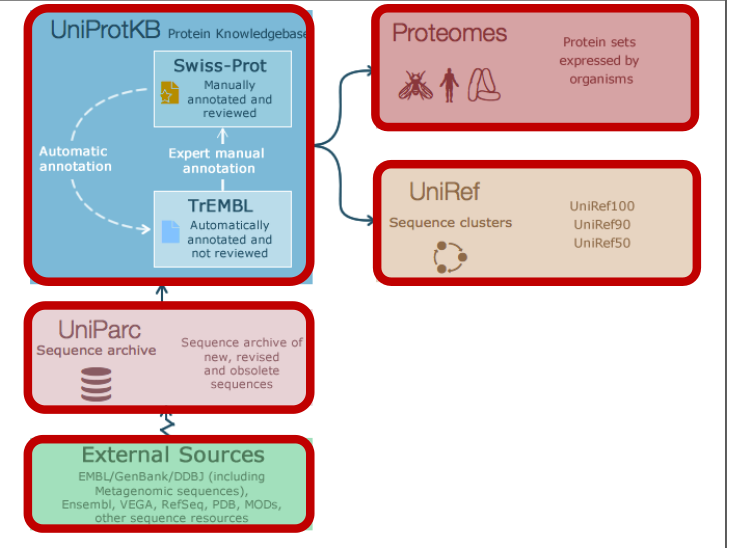
\includegraphics[width=.9\linewidth]{UniProt/uniprot_scheme_2020-11-17_15-52-59.png}
\caption{UniProt Scheme}
\end{figure}


I very important understand which UniProt Release we are using.


\subsection{Manual Curation* (it is a process of \underline{validation})}
\label{sec:orgad5bea2}
\emph{Manual curation} consists of a critical review of experimental and predicted data
for each protein as well as manual verification of each protein sequence.
Curation methods applied to UniProtKB/Swiss-Prot include
\begin{itemize}
\item manual extraction and structuring of information from the literature
\item manual verification of results from computational analyses
\item mining and integration of large-scale data sets
\item continuous updating as new information becomes available.
\end{itemize}



\textbf{Discrepancies between sequence reports} are identified, with underlying causes such as:
\begin{itemize}
\item alternative splicing
\item natural variations
\item frameshifts
\item incorrect initiation sites
\item incorrect exon boundaries
\item unidentified conflicts
\item erroneous gene prediction
\end{itemize}

\textbf{Comparison with homologous sequences} can be used to identify sequence errors
and their causes. Each protein in Swiss-Prot should be as complete and correct as possible.

\textbf{Annotations}\\
\begin{itemize}
\item Biological Process
\item Molecular Function : Activity or task performed
\item Cellular Component : Where is the protein located
\end{itemize}


\subsection{Gene ontology}
\label{sec:org9b1e2b4}
An ontology is a formal representation of a body of knowledge within a given domain.
Ontologies usually consist of a set of classes (or terms or concepts) with relations that
operate between them.

The Gene Ontology (GO) describes our knowledge of the biological domain with respect to three
aspects:
\begin{itemize}
\item \emph{Molecular function} : Molecular-level activities performed by gene products. Molecular
function terms describe activities that occur at the molecular level, such as “catalysis” or
“transport”. GO molecular function terms represent activities rather than the entities
(molecules or complexes) that perform the actions, and do not specify where, when, or in
what context the action takes place. Molecular functions generally correspond to activities
that can be performed by individual gene products (i.e. a protein or RNA).

\item \emph{Cellular Component} : The locations relative to cellular structures in which a gene product
performs a function, either cellular compartments (e.g., mitochondrion), or stable
macromolecular complexes of which they are parts (e.g., the ribosome).

\item \emph{Biological Process} : The larger processes, or ‘biological programs’ accomplished by
multiple molecular activities. Examples of broad biological process terms are DNA repair or
signal transduction. Examples of more specific terms are pyrimidine nucleobase biosynthetic
process or glucose transmembrane transport.
\end{itemize}

\subsubsection{GO Classes}
\label{sec:org6a1eee4}
GO classes (or GO terms) are composed of a definition, a label, a unique identifier, and
several other elements.

\uline{Required fields}\\
\begin{itemize}
\item Unique Identifier (ID)
\item Term Human Readable name
\item Aspect : which of the three ontologies does this entity belong to
\item Definition: textual definition of what the terms represent
\item Relationship with other terms
\end{itemize}

\uline{Optional elements}\\
\begin{itemize}
\item Secondary ID
\item Synonyms
\item Comments
\item DB cross reference
\end{itemize}

\subsubsection{Go domains and graph}
\label{sec:org9cd3ae9}
The three GO domains (cellular component, biological process, and molecular function) are each
 represented by a separate root ontology term. All terms in a domain can trace their parentage
 to a root term, although there may be numerous different paths via varying numbers of
 intermediary terms to a ontology root. The three root nodes are unrelated and do not have a
 common parent node, and hence GO is three ontologies.
\url{file:///home/codicef/bioinformatics-notes/Bioinformatics\_Lab1/Functional Annotation/ggaagaga\_2020-12-20\_15-42-29.gif}

\subsubsection{Go annotations}
\label{sec:orgcf542d0}
A GO annotation is a statement about the function of a particular gene. GO annotations are
created by associating a gene or gene product with a GO term.

Together, these statements comprise a “snapshot” of current biological knowledge. Hence, GO
annotations capture statements about how a gene functions at the molecular level, where in the
cell it functions, and what biological processes (pathways, programs) it helps to carry out.

There are four pieces of information that uniquely identify a GO annotation. Although there
are additional components a curator can use to indicate more information, including qualifiers
and annotation extensions, at the very minimum an annotation consists of:

\begin{itemize}
\item Gene product (may be a protein, RNA, etc.)
\item GO term
\item Reference
\item Evidence
\end{itemize}


\subsection{UniProt Annotation System}
\label{sec:org1d595bb}

\textbf{Enzyme Classification} (6 CLASSES)
\begin{center}
\begin{tabular}{rl}
EC Class & Reaction Type\\
1 & Oxidoreductases\\
2 & Trannsferases\\
3 & Hydrolases\\
4 & Lyases\\
5 & Isomerases\\
6 & Ligases\\
\end{tabular}
\end{center}

This is a tree like classification. It is used a 4 numbers code to annotate an enzyme.

\begin{figure}[htbp]
\centering
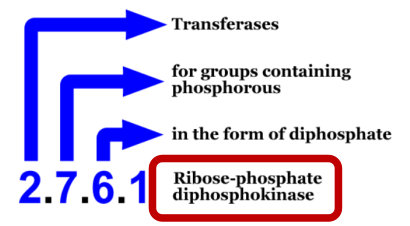
\includegraphics[width=.9\linewidth]{UniProt/enzyme_annotation_2020-11-17_16-33-10.png}
\caption{Annotation of Enzyme}
\end{figure}


\begin{itemize}
\item \textbf{UniProtKB/TrEMBL}
\begin{itemize}
\item Redundant
\begin{itemize}
\item 1 entry for each translated ENA entry
\item Computationally analyzed
\item Automatically annotated
\item Unreviewed
\end{itemize}
\end{itemize}
\end{itemize}


\textbf{ARBA (Association rule based annotation)} : uses rule mining techniques to generate 
annotation models, based on the InterPro classification.



\begin{itemize}
\item \textbf{UniProtKB/SwissProt}
\begin{itemize}
\item Non-Redundant
\begin{itemize}
\item 1 entry for each protein
\item Curator analyzed
\item High-quality manually annotated
\item Reviewed
It is safe to assume that manual annotations are more reliable than automatic ones.
\textbf{UniRule}: maintains a set of manually established annotation rules.

\textbf{InterPro} is an effort to integrate all the main databases about protein classification.
\end{itemize}
\end{itemize}
\end{itemize}

\begin{figure}[htbp]
\centering
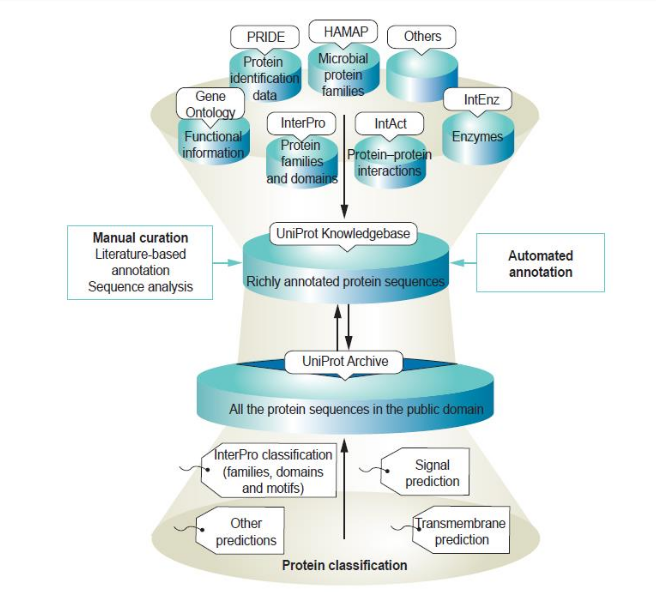
\includegraphics[width=.9\linewidth]{UniProt/annotation_workflow_2020-11-17_16-59-14.png}
\caption{Annotation Sources used by curators}
\end{figure}


\subsubsection{Evidence And Conlcusion Ontology}
\label{sec:org47859cf}
An \textbf{evidence} is described by a type (mandatory evidence type), represented by a code from
the Evidence and Conclusion Onthology(ECO) and ,if available, the source of the information,
which is usually a database record.

\textbf{Example}
\begin{itemize}
\item Evidence type without source\{type\}
\begin{verbatim}
{ECO: 0000305}
{ECO: 000250}
{ECO: 000255}
\end{verbatim}

\item Evidence type with source \{type|source\}
\begin{verbatim}
{ECO: 0000305|Pubmed:2435555}
{ECO: 000250|UniProtKB:p11497}
\end{verbatim}
\end{itemize}

\begin{figure}[htbp]
\centering
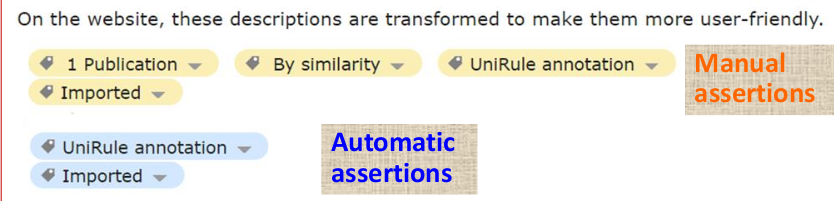
\includegraphics[width=.9\linewidth]{UniProt/manual_auto_annotations_2020-11-17_16-55-28.png}
\caption{Annotation format/style on Uniprot}
\end{figure}


\subsubsection{Annotations categories}
\label{sec:org36edd3c}
\begin{itemize}
\item Function
\item Names \& Taxonomy
\item Subcellular location
\item Pathology \& Biotech
\item Post Translation Modifications / Processing
\item Expression
\item Interactions
\item Structure
\item Family and Domains
\item Sequences
\item Similar Proteins
\item Cross-referenes
\item Entry informations
\end{itemize}


\subsubsection{Automatic Annotation}
\label{sec:org9de44d0}
\begin{center}
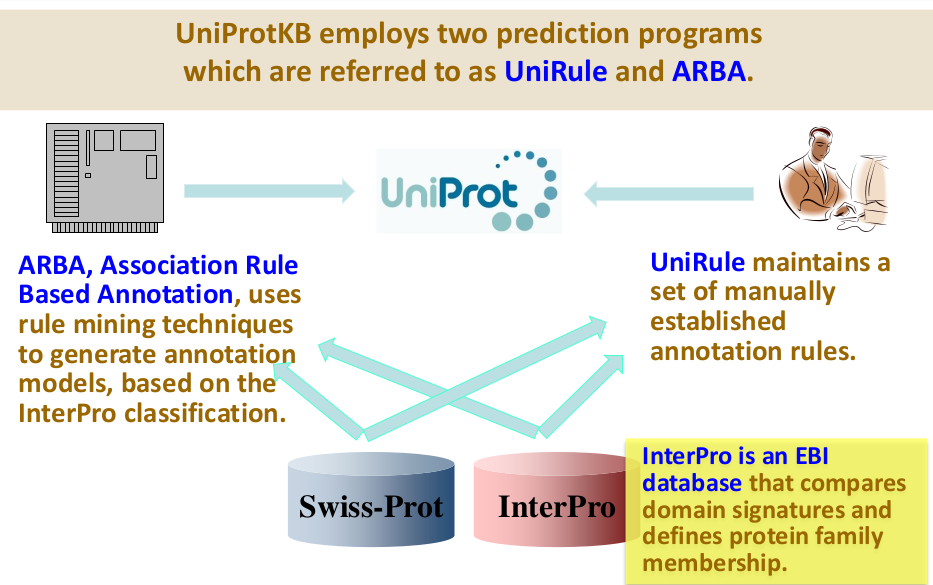
\includegraphics[width=.9\linewidth]{imgs/UniProt/2021-02-01_18-24-09_screenshot.png}
\end{center}


\textbf{Problems}\\
Electronic Annotation follows the principle that proteins with similar sequences
and similar structures frequently carry out similar functions.

But protein sequence or structure similarity alone does not necessarily equate
to cellular or molecular functional similarity.

\subsubsection{Annotation Score}
\label{sec:org46eb451}
The annotation score provides a heuristic measure of the annotation content of a
UniProtKB entry or proteome. This score cannot be used as a measure of the
accuracy of the annotation as we cannot define the 'correct annotation' for any
given protein.

The annotation score is computed in the following way:

\begin{itemize}
\item Different UniProtKB annotation types (e.g. protein names, gene names, functional annotations (comments) and sequence annotations (features), GO annotations, cross-references) are scored either by presence or by number of occurrences.

Annotations with experimental evidence score higher than equivalent
predicted/inferred annotations, thereby favoring expert literature-based
curation over automatic annotation.

\item The score of an individual entry is the sum of the scores of its annotations.

\item The score of a proteome is the sum of the scores of the entries that are part of the proteome.
\end{itemize}


\subsection{Interpro Database}
\label{sec:org073fced}
InterPro is a database of \uline{protein families, domains and functional sites} in which identifiable features found in known proteins can be applied to new protein sequences in order to functionally characterise them.

The contents of InterPro consist of diagnostic signatures and the proteins that
they significantly match. The \uline{signatures consist of models} (\emph{simple types,
such as regular expressions or more complex ones, such as Hidden Markov models})
which describe \emph{protein families}, \emph{domains} or \emph{sites}.

Models are built from the amino acid sequences of known families or domains and
they are subsequently used to search unknown sequences (such as those arising
from novel genome sequencing) in order to classify them.


\begin{itemize}
\item In InterPro, patterns, profiles, fingerprints and HMMs from a number of
different databases are brought together into a single searchable resource.
\end{itemize}

\begin{center}

\includegraphics[width=.9\linewidth]{imgs/UniProt/2021-02-01_18-38-27_screenshot.png}
\end{center}


\subsection{Uniprot Entry}
\label{sec:orge593921}
Annotations of a UniProtKB entry are structured into the following sections:
\begin{itemize}
\item Function
\item Names \& Taxonomy
\item Subcellular location
\item Pathology and Biotech
\item PTM / Processing
\item Expression
\item Interaction
\item Structure
\item Family and Domains
\item Sequence(s)
\item Cross-references
\item Publications
\item Entry information
\item Miscellaneous
\item Similar Proteins
\end{itemize}




\subsection{UniParc}
\label{sec:orgd257bdb}
UniProt Archive (UniParc): An archive for tracking protein sequences
\begin{itemize}
\item Comprehensive : contains most of the publicly available protein sequences in
the world
\item Non-redundant : merges identical sequence strings, each unique sequence is
given a stable and unique identifier (UPI)
\item Traceable : Versioned, with ‘active’ and ‘obsolete’ status tags
\item Concise : no annotations
\end{itemize}


\subsection{UniRef}
\label{sec:orgde829cc}
The \emph{UniProt Reference Clusters (UniRef)} provide clustered sets of sequences from the UniProt Knowledgebase (including isoforms) and selected UniParc records in order to obtain complete coverage of the sequence space at several resolutions while hiding redundant sequences (but not their descriptions) from view.

\textbf{UniRef Cluters}\\
\begin{itemize}
\item \emph{UniRef50} : UniRef50 is generated by clustering UniRef90 seed sequences that
have at least 50\% sequence identity.

\item \emph{UniRef90} : UniRef90 is generated by clustering UniRef100 seed sequences that
have at least 90\% sequence identity.

\item \emph{UniRef100} : UniRef100 contains all UniProt Knowledgebase records plus selected UniParc records (see below). It is generated by clustering identical sequences and subfragments.
\end{itemize}


\begin{center}
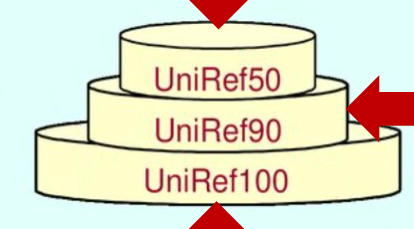
\includegraphics[width=.9\linewidth]{imgs/UniProt/2021-02-04_11-15-31_screenshot.png}
\end{center}

\subsubsection{UniRef Seed}
\label{sec:org2eb5360}
\begin{itemize}
\item A UniRef seed is the sequence that has been used as the template to recruit
other sequences by the clustering algorithm. The seed sequence is the longest
member of a cluster.
\item However, the longest sequence is not always the most informative one. There is
often more biologically relevant information (name, function,
cross-references) available on other cluster members. Therefore, in addition,
a \emph{representative sequence is chosen for each cluster}.
\end{itemize}


\subsection{Proteomes}
\label{sec:orga48c539}
A proteome is the set of proteins thought to be expressed by an organism.
UniProt provides proteomes for species with completely sequenced genomes

\begin{itemize}
\item \emph{Reference Proteomes} : Some proteomes have been (manually and
algorithmically) selected as reference proteomes. They cover well-studied
model organisms and other organisms of interest for biomedical research and
phylogeny
\end{itemize}


\begin{figure}[htbp]
\centering
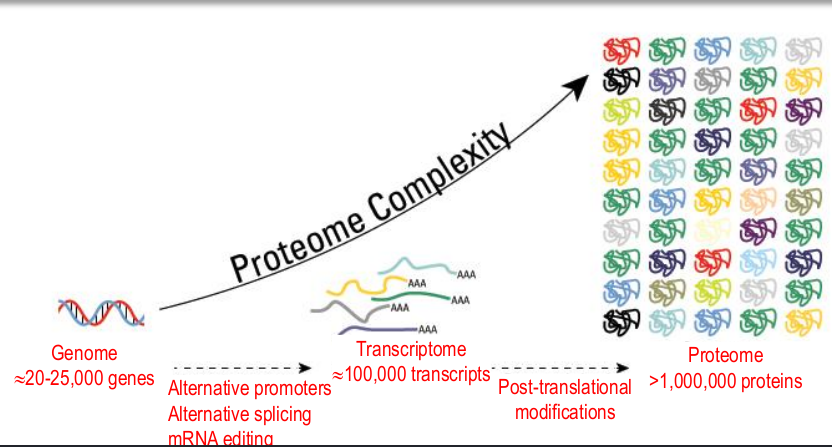
\includegraphics[width=.9\linewidth]{imgs/UniProt/2021-02-04_11-19-25_screenshot.png}
\caption{Proteome Complexity}
\end{figure}


\subsubsection{Human Proteome}
\label{sec:org3556cf5}
September 2008 First draft of the complete human proteome available in
UniProtKB/ Swiss-Prot. Gene prediction algorithms, plus the existing transcript
and protein information, have enabled the identification of most exons in a
genome.



\subsection{Protein Classification}
\label{sec:org0accf95}
\textbf{Protein Family}\\
A protein family is a group of proteins that share a common evolutionary origin,
reflected by their related functions and similarities in sequence or structure.
Protein families are often arranged into hierarchies.


\begin{figure}[htbp]
\centering
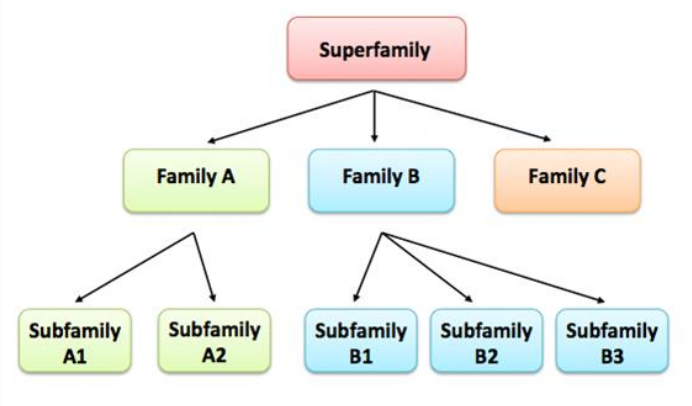
\includegraphics[width=.9\linewidth]{UniProt/proteinfamilies_2020-11-24_15-05-42.png}
\caption{Protein families}
\end{figure}



\begin{center}
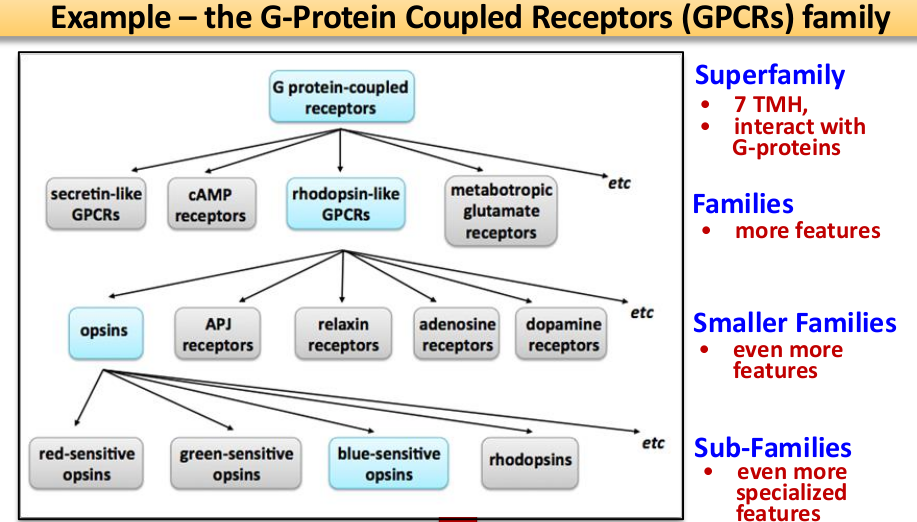
\includegraphics[width=.9\linewidth]{UniProt/proteinfaimilies%20example_2020-11-24_15-07-35.png}
\end{center}





\textbf{Protein Domains} 

A protein domain is a conserved part of a given protein sequence and tertiary structure that
can evolve, function, and exist independently of the rest of the protein chain. Each domain

Domains have been described as units of: 
\begin{itemize}
\item compact structure
\item function and evolution
\item folding
\end{itemize}

Each of these definition is valid and will often overlap. The identification of
domains that occur within proteins can provide insights into their function.



\textbf{Protein Signatures}
Signatures: mathematical models constructed from MSA.
They are often a very sensitive way of identifying protein function.
\begin{figure}[htbp]
\centering
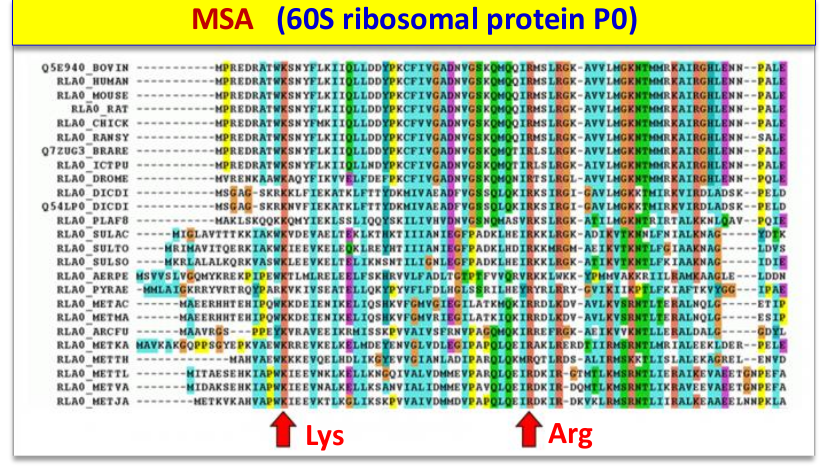
\includegraphics[width=.9\linewidth]{UniProt/signatures_2020-11-24_15-25-48.png}
\caption{Protein Signatures}
\end{figure}


\textbf{Protein Profile}




\subsubsection{InterPro database}
\label{sec:org3f6e8e5}
In InterPro, patterns, profiles, fingerprints and HMMs from a number of different databases
are brought together into a single searchable resource.
\begin{figure}[htbp]
\centering
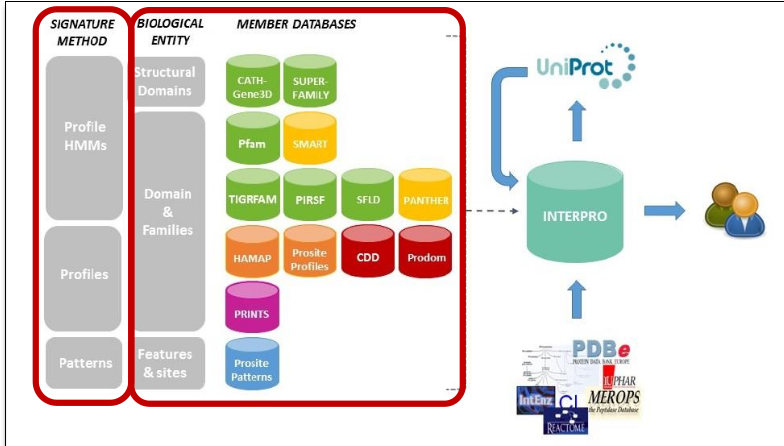
\includegraphics[width=.9\linewidth]{UniProt/interpro_2020-11-24_15-36-03.png}
\caption{Interpro scheme}
\end{figure}


\subsubsection{PFam Database}
\label{sec:org70e2619}
\begin{figure}[htbp]
\centering
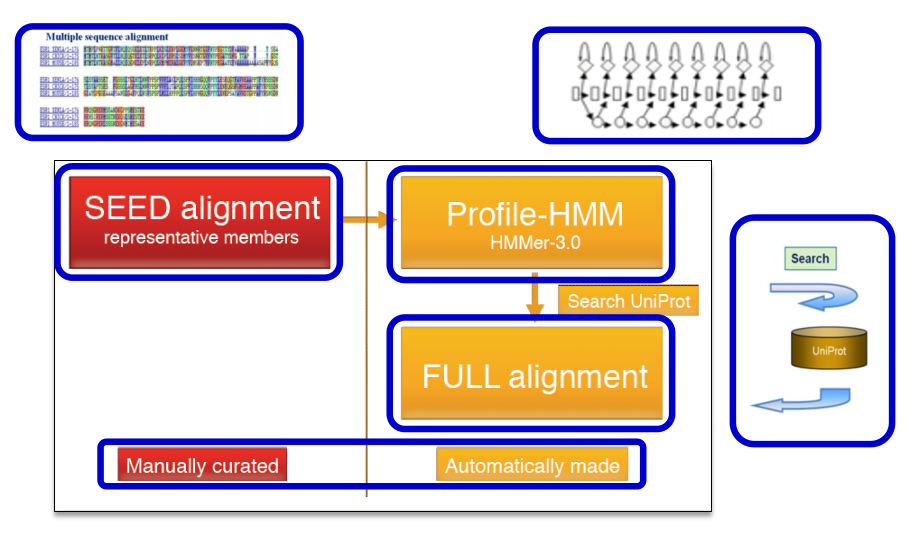
\includegraphics[width=.9\linewidth]{UniProt/pfam_2020-11-24_15-39-01.png}
\caption{Pfam}
\end{figure}



\subsection{Exercises}
\label{sec:orgedc7583}
\subsubsection{Exercise 1}
\label{sec:orgdfe5d1e}
\begin{itemize}
\item \textbf{Question} : Write down a single query which will retrieve within UniProt all proteins, labelled as proteases in the CC function field, from human and mouse, excluding those labelled as ``cysteine proteases'' in the same field.

\item \textbf{Answer}
\end{itemize}
\#+BEIN\textsubscript{SRC}
annotation:(type:function protease) (organism:``Homo sapiens (Human) [9606]'' OR organism:``Mus musculus (Mouse) [10090]'') NOT annotation:(type:function ``cysteine protease'')
\#+END\textsubscript{SRC}

\subsubsection{Exercise 2}
\label{sec:org679c560}
\begin{itemize}
\item \textbf{Question}
\end{itemize}
Do the same as above, but using the EC codes for ``proteases'' and for ``cysteine proteases''.

\begin{itemize}
\item \textbf{Answer}
\begin{verbatim}
ec:3.4.*.* NOT ec:3.4.22.* (organism:"Homo sapiens (Human) [9606]" OR organism:"Mus musculus (Mouse) [10090]")
\end{verbatim}
\end{itemize}

\subsubsection{Exercise 3}
\label{sec:org195ce25}
\begin{itemize}
\item \textbf{Question} :
Which protein is involved in the human sma2 disease ? (insert UniProt code)

\item \textbf{Answer}
\begin{verbatim}
  annotation:(type:disease sma2) AND organism:"Homo sapiens (Human) [9606]"
\end{verbatim}

Q16637 (\url{https://www.uniprot.org/uniprot/Q16637})
\end{itemize}

\subsubsection{Exercise 4}
\label{sec:orgc116e85}
\begin{itemize}
\item \textbf{Question}
\begin{itemize}
\item Which natural variant reduces in the sma2 and sma3 disease the binding of such protein to RPP20/POP7?  Which is the corresponding dbSNP code? (insert UniProt variant code and dbSNP code)
\item On which evidence is the above piece of information based? Which is the
UniProt code for the evidence type?
\end{itemize}
\item \textbf{Answer}
Search in pathology and biotech sections
\begin{itemize}
\item \uline{Natural variant VAR\textsubscript{005618}}   \uline{dbSNP:rs76871093}
\item Experimental ,  ECO:0000269
\end{itemize}
\end{itemize}

\subsubsection{Exercise 5}
\label{sec:org1c9f9f0}
\begin{itemize}
\item \textbf{Question}

\item \textbf{Answer}
UP000005640 <- Proteome id
\begin{itemize}
\item 75,777 <- Proteins present
\item 602 <- Uncertain proteins
\begin{verbatim}
    existence:"Uncertain [5]" AND organism:"Homo sapiens (Human) [9606]" AND proteome:up000005640
\end{verbatim}
\end{itemize}
\end{itemize}

\section{ENSEMBL}
\label{sec:orgfda85e6}
Ensembl is a joint project between the European Bioinformatics Institute and the
Wellcome Trust Sanger Institute, launched in 1999 in response to the imminent
completion of the Human Genome Project.

\begin{itemize}
\item The Ensembl project team developed new software pipelines to automatically
generate evidence-based annotation of genome sequences.
\item The Ensembl project has expanded from the curation of the human genome to
embrace more than 50 vertebrate species, and several hundreds non vertebrates
species.
\item Generating the annotation is just the start. Ensembl provides several means of
data access, the foremost of which is a highly customisable, interactive
website.
\end{itemize}

\subsection{ENSEMBL Features}
\label{sec:orga09e66d}
\begin{itemize}
\item The gene set
\begin{itemize}
\item Splice variant, proteins, noncoding RNA
\end{itemize}
\item Comparative analysis
\begin{itemize}
\item Whole genome alignments, protein trees
\end{itemize}
\item Variation and regulation
\begin{itemize}
\item Variants (SNPs, InDels, CNVs)
\end{itemize}
\item BioMart (data export)
\item Programmatic access via Perl-API, MySQL
\item Data and code are open source
\end{itemize}


\subsection{Human Genome}
\label{sec:orgb1ff8e2}
The human genome consists of three billion base pairs, which code for approximately \emph{20,000–25,000} genes.

\begin{itemize}
\item However the genome alone is of little use, unless the locations and relationships of individual genes can be identified. One option is manual annotation, whereby a team of scientists tries to locate genes using experimental data from scientific journals and public databases. However this is a slow, painstaking task.
\item The alternative, known as automated annotation, is to use the power of computers to do the complex pattern-matching of protein to DNA.
\end{itemize}



\begin{center}
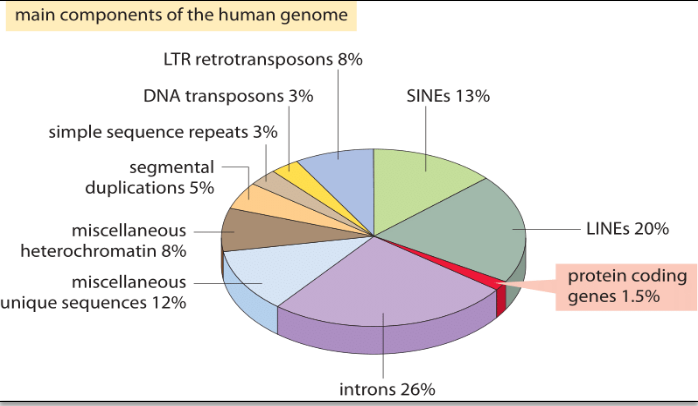
\includegraphics[width=.9\linewidth]{imgs/ENSEMBL/2021-02-05_10-43-08_screenshot.png}
\end{center}

About 1.5\% of the genome consists of the \(\simeq 20,000\) protein-coding sequences which
are interspersed by the non coding introns ( \(\simeq 26%\) ). Transposable Elements are
the largest fraction (40-50\%) including for example Long Interspersed Nuclear
Elements (LINEs), and Short Interspersed Nuclear Elements (SINEs). Most
Transposable Elements are genomic remnants, which are currently defunct.


\textbf{Transcribed Human Genome}
\begin{center}
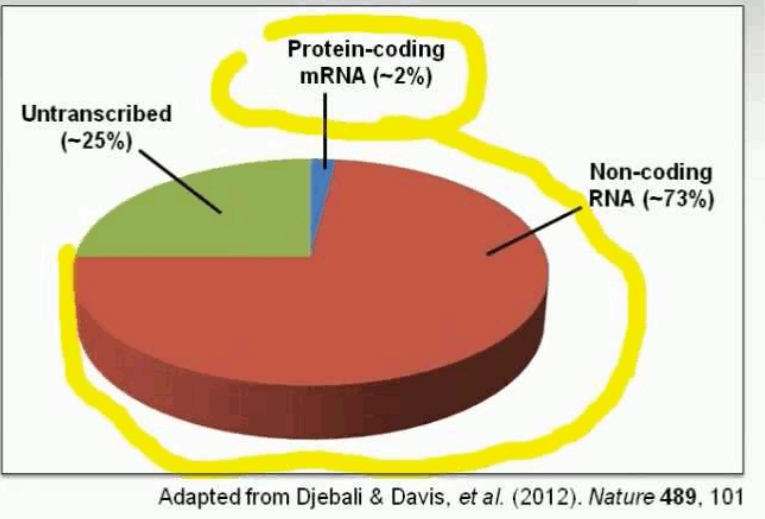
\includegraphics[width=.9\linewidth]{imgs/ENSEMBL/2021-02-05_10-44-54_screenshot.png}
\end{center}

\subsubsection{Gene Quantification}
\label{sec:orge8521e0}
A comparison between the number of genes in an organism and a naïve estimate
based on the genome size divided by a constant factor of 1000bp/gene.

It is found that this crude rule of thumb, which works well for many bacteria
and archaea, fails for multicellular organisms.

\begin{center}
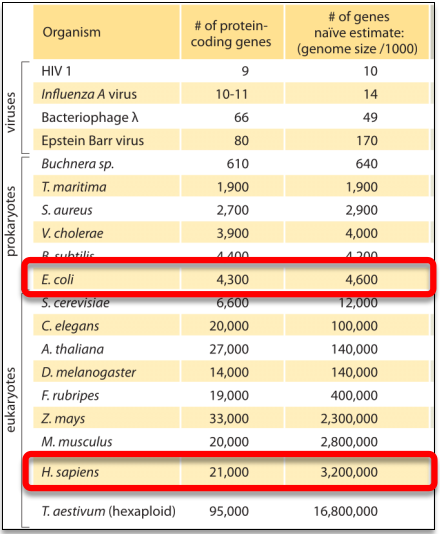
\includegraphics[width=.9\linewidth]{imgs/ENSEMBL/2021-02-05_10-46-53_screenshot.png}
\end{center}






\subsection{Gene Prediction}
\label{sec:orgced4c3a}
\begin{center}
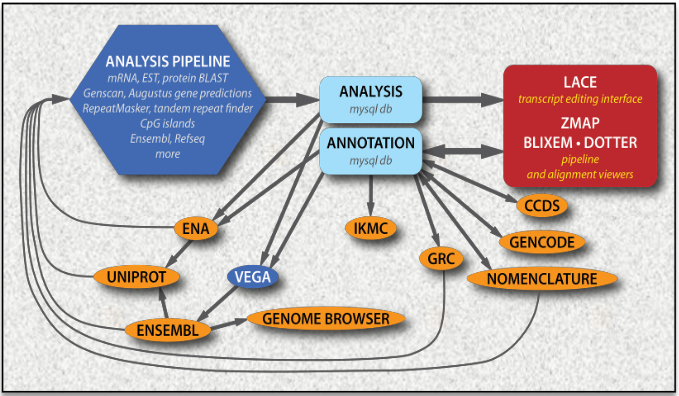
\includegraphics[width=.9\linewidth]{imgs/ENSEMBL/2021-02-05_10-54-04_screenshot.png}
\end{center}

\textbf{Automatic Annotation}\\
Gene building all at once (whole genome) → «Ensembl»
\begin{itemize}
\item cDNA and protein alignments (from sequence DBs)
\item RNAseq data
\item Ab initio predictions (based on the genomic sequence, no experimental
evidence)
\item Gene predictions based on ESTs (ESTGenes)
\end{itemize}


\textbf{Manual Annotation}\\
Gene determination on a case-by-case by a curator →
\begin{itemize}
\item VEGA (VErtebrate Genome Annotation)
\item Havana (Human And Vertebrate ANalysis and Annotation)
\end{itemize}

\subsection{Ensembl vs Havana}
\label{sec:orgf21cce8}

\begin{center}
\begin{tabular}{ll}
ENSEBL & Havana\\
\hline
Automatic Annotation & Manual Annotation\\
Many Species(n=61) & Fewer Species\\
Genome-wide at once & Gene by gene\\
\end{tabular}
\end{center}


When Havana and Ensembl predict the same transcript, basepair for basepair, the
transcripts are merged and coloured gold


\begin{itemize}
\item A protein is deposited into the \emph{``Consensus CDS protein set''} (CCDS set) if
NCBI, UCSC, Havana, Ensembl have determined the same sequence.
\end{itemize}

\subsection{Glossary}
\label{sec:org8082b03}
\subsubsection{Locating a gene}
\label{sec:orga54d42b}

The cytogenetic location, a standardized way of describing a gene’s location on the chromosome, consists of a combination of numbers and letters and is made up of three components:

Number or letter of the chromosome (1-23, X or Y)

Arm of the chromosome (p or q)

Position of the gene on the arm (cytogenetic bands). The position is dependent on the light and dark bands that appear on the chromosome when stained and is expressed as a two-digit number (one digit represents region and one represents band). Sometimes the digits are followed by a decimal point and one or more digits. These additional digits represent the distance from the centromere (increasing numeric value indicates farther distance from centromere). “Cen”, “ter”, and “tel” are also used to describe the position of the gene on the arm.

Cen – close to the centromere
Ter (terminus) – close to end of either the p or q arms
Tel (telomere) – close to end of either the p or q arms

Example
Gene: Anaplastic lymphoma kinase receptor
Chromosomal location: 2p23
Location description: chromosome 2, p arm, position 23

\subsection{Exercises}
\label{sec:org479623d}
\subsubsection{Exercise ENSEMBL}
\label{sec:org7a869a2}
\begin{itemize}
\item \textbf{Question}\\
The LCT gene product (lactase) has lactase activity. Mutations in this gene
are associated with congenital lactase deficiency. Polymorphisms in this
gene are associated with lactase persistence, in which intestinal lactase
activity persists at childhood levels into adulthood.
\begin{enumerate}
\item Which is the Ensembl code for this gene? How many transcripts are reported
for this gene? Are they all protein coding? Are they coded on the forward
or reverse strand?
\item Which is the Ensembl code of the longest transcript? Which is its CCDS code
? And its Refseq codes ?
\item Which are the chromosomal coordinates of this gene ? And its cytogenetic
location ?
\item Which is the protein sequence in the reference genome between positions 2: 135,829,587  and 2:135,829,598 ? Are there variants for these residues,
which are annotated in Ensembl ? Which databases do they come from ? What
are their amino acid positions, in the protein product from the LCT-201
transcript ?
\end{enumerate}

\item \textbf{Answer}\\
\begin{enumerate}
\item The Ensembl code is \emph{ENSG00000115850} . This gene has 2 transcripts.
LCT-201 yes, LCT-202. Reverse strand for both.

\item ENST00000264162.7 . CCDS2178 . NM\textsubscript{002299.4}

\item Chromosome 2: 135,787,850-135,837,184 . q21.3

\item LCT-201, yes, dbSNP, 801, 817
\end{enumerate}
\end{itemize}


\section{PDB}
\label{sec:org23d3916}
It is an archive of \emph{experimentally determined} 3-dimensional structures of biological 
macro-molecules (Protein, nucleic acids, sugars).

The PDB is a key in areas of structural biology, such as structural genomics.
Most major scientific journals, and some funding agencies, now require
scientists to submit their structure data to the PDB.


\textbf{Content}
\begin{itemize}
\item \emph{X-ray Crystallography} (88\%) : Strucure Factors data
\item \emph{NMR Spectroscopy} (10\%) : Restrains, Chemical Shifts
\item \emph{Electron Microscopy} (1\%) : Map in EMDB
\end{itemize}

\#+CAPTION : PDB History
\begin{center}
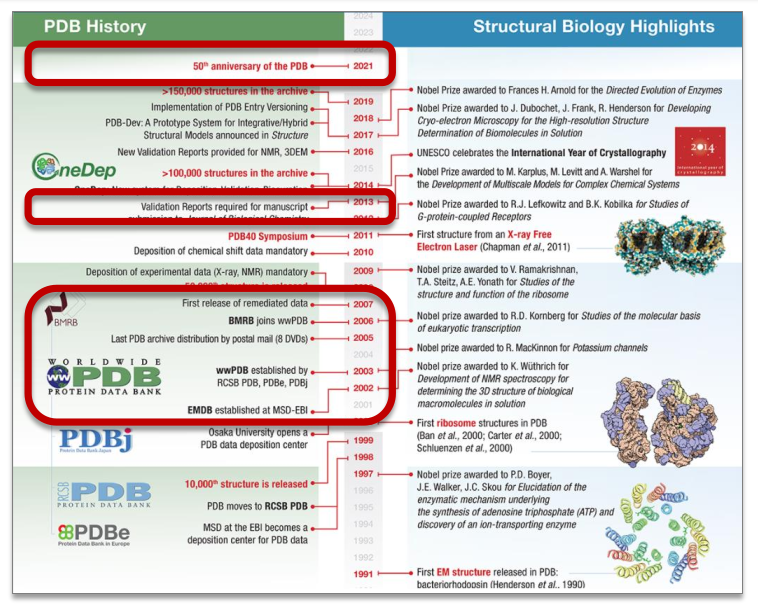
\includegraphics[width=.9\linewidth]{PDB/pdbhistory_2020-12-03_14-51-02.png}
\end{center}

\subsection{Validation}
\label{sec:org14c629d}
\textbf{Validation side}\\
Method-specific Validation Task Forces have been convened to
collect recommendations and develop consensus on additional validation that
should be performed, and to identify software applications to perform validation
tasks. There are tools available for the validation of X-ray Crystallography, NMR and
Electron Microscopy data.

There are many metrics used to validate the quality of a protein structure in the PDB file.

\subsubsection{B-Factor (Temperature Factor)}
\label{sec:org7de7689}
The \emph{B-factor} for each atom is given by: \(B = 8 \pi^{2} U^{2}\)
where \(U^{2}\) is the \emph{mean square displacement} of the atom.

\emph{Mean Square Displacement} : It is the most common measure of the spatial extent
of random motion, and can be thought of as measuring the portion of the system
``explored'' by the random walker.

Examples
if B-factor = 15 A -> mean square displacement \(\simeq 0.44 A\)
if B-factor = 60 A -> mean square displacement \(\simeq 0.87 A\)

\textbf{Methods}\\
\begin{itemize}
\item \textbf{Resolution} : Resolution in X-ray crystallography: the highest resolvable peak
in the diffraction pattern. If the proteins in the crystal are not perfectly aligned, but
all slightly different, due to local flexibility or disorder, the diffraction pattern will
not show such fine information.

High-resolution structures, with resolution values of 1 Å or so, are highly
ordered and it is easy to see every atom in the electron density map. Lower
resolution structures, with resolution of 3 Å or higher, show only the basic
contours of the protein chain, and the atomic structure must be inferred. Most
crystallographic-defined structures of proteins fall in between these two
extremes.

\begin{center}
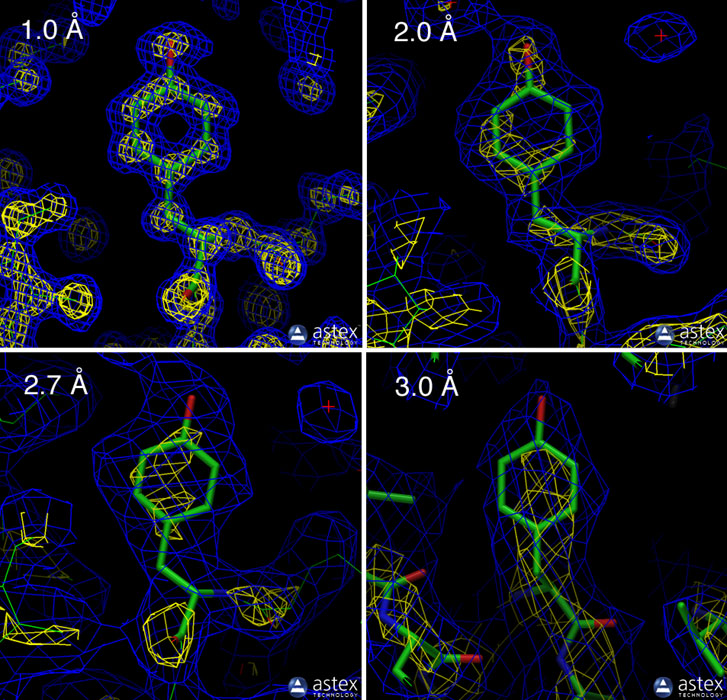
\includegraphics[width=.9\linewidth]{PDB/resolution-figure_2020-12-05_11-58-05.jpg}
\end{center}

\item \textbf{R-value} (x-ray only): \emph{R-value} is the measure of the quality of the atomic model obtained from the
crystallographic data. When solving the structure of a protein, the researcher first builds
an atomic model and then calculates a simulated diffraction pattern based on that model. 

The R-value measures how well the simulated diffraction pattern matches the
experimentally-observed diffraction pattern. 

A totally random set of atoms will give an R-value of about 0.63, whereas a perfect fit
would have a value of 0. Typical values are about 0.15-0.20.
\end{itemize}



\begin{itemize}
\item \textbf{R-free} (x-ray only) : There is one potential problem with using R-values to assess the quality of a
structure. The refinement process is often used to improve the atomic model of a given
structure to make it fit better to the experimental data and improve the R-value.
Unfortunately, this introduces bias into the process, since the atomic model is used along
with the diffraction pattern to calculate the electron density. 

The use of the R-free value is a less biased way to look at this. Before refinement begins,
about 10\% of the experimental observations are removed from the data set. Then, refinement
is performed using the remaining 90\%. The R-free value is then calculated by seeing how well
the model predicts the 10\% that were not used in refinement.

\item \textbf{RSRz} (x-ray only) : The real-space R-value (RSR) is a measure of the quality of fit between a part of
an atomic model (in this case, one residue) and the data in real space (Jones et al., 1991).
The RSR Z-score (RSRZ) is a normalisation of RSR specific to a residue type and a resolution
bin (Kleywegt et al., 2004). RSRZ is calculated only for standard amino acids and
nucleotides in protein, DNA and RNA chains.

\item \textbf{Ramachandran Outlier} (all methods): A residue is considered to be a Ramachandran plot outlier if the
combination of its φ and ψ torsion angles is unusual, as assessed by MolProbity (Chen et
al., 2010). The Ramachandran outlier score for an entry is calculated as the percentage of
Ramachandran outliers with respect to the total number of residues in the entry for which
the outlier assessment is available.
\item \textbf{Clashscore} (all methods): Atoms bumping into each other score
\item \textbf{Sidechain Outlier} (all methods): Protein sidechains mostly adopt certain (combinations of) preferred
torsion angle values (called rotamers or rotameric conformers), much like their backbone
torsion angles (as assessed in the Ramachandran analysis). MolProbity considers the
sidechain conformation of a residue to be an outlier if its set of torsion angles is not
similar to any preferred combination. The sidechain outlier score is calculated as the
percentage of residues with an unusual sidechain conformation with respect to the total
number of residues for which the assessment is available.
\end{itemize}


\textbf{Percentile Slider}\\
The metrics shown in the ``slider'' graphic (see examples below) compare several important
global quality indicators for this structure with those of previously deposited PDB entries.
The comparison is carried out by calculation of the percentile rank, i.e. the percentage of
entries that are equal or poorer than this structure in terms of a quality indicator. The
global percentile ranks (black vertical boxes) are calculated with respect to all X-ray
structures available in the PDB archive
\begin{center}
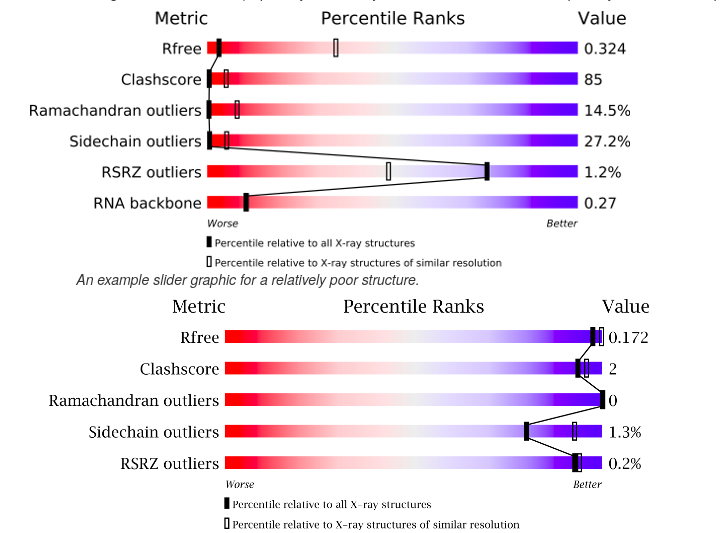
\includegraphics[width=.9\linewidth]{PDB/validation_2020-12-05_15-46-08.png}
\end{center}


\textbf{Chain quality details graph}\\
\begin{center}
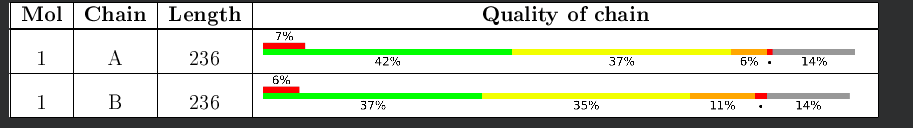
\includegraphics[width=.9\linewidth]{PDB/polymericchain_2020-12-05_16-23-51.png}
\end{center}

There may be green, yellow, orange and red portions in the lower bar for each chain,
indicating the fraction of residues that contain outliers for 0, 1, 2, ≥3 model-only
validation criteria, respectively. A grey segment indicates residues present in the sample but
not modelled in the final structure. If electron density outliers were present, there is an
additional red bar above the lower bar, indicating the fraction of residues that are RSRZ
outliers.




\textbf{NMR validation}\\
\begin{center}
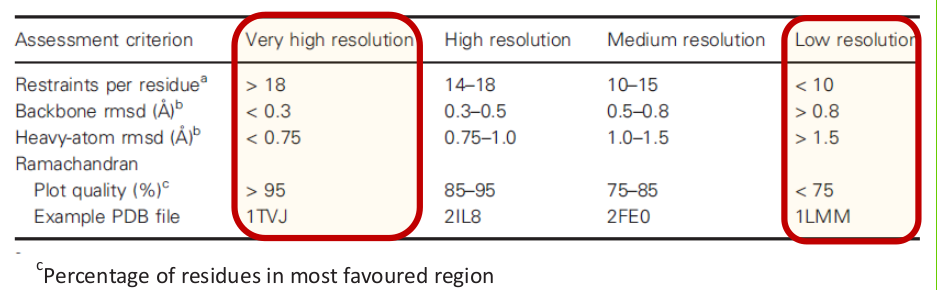
\includegraphics[width=.9\linewidth]{PDB/nmr_2020-12-05_16-04-30.png}
\end{center}


\textbf{Crio-electron microscopy}\\
From Neumann et al. 2018 : Recent advances in instrumentation and image-processing software
have resulted in a resolution revolution in cryo-electron microscopy \ldots{}. However despite
technical progress and hundreds of structures determined so far, development of standards
assessing the agreement between the cryo-em map and the respective model as fallen behind. 


\subsection{PDB File Format}
\label{sec:orge77b6af}
The Protein Data Bank (pdb) file format is a textual file format describing the
three-dimensional structures of molecules held in the Protein Data Bank. The pdb
format accordingly provides for description and annotation of protein and
nucleic acid structures including atomic coordinates, secondary structure
assignments, as well as atomic connectivity. In addition experimental metadata
are stored.

\begin{itemize}
\item \emph{HEADER}, \emph{TITLE} and \emph{AUTHOR} records provide information about the researchers who
defined the structure; numerous other types of records are available to
provide other types of information.
\item \emph{REMARK} records can contain free-form annotation, but they also accommodate
standardized information; for example, the REMARK 350 BIOMT records describe
how to compute the coordinates of the experimentally observed multimer from
those of the explicitly specified ones of a single repeating unit.
\item \emph{SEQRES} records give the sequences of the three peptide chains (named A, B
and C), which are very short in this example but usually span multiple lines.
\item \emph{ATOM} records describe the coordinates of the atoms that are part of the
protein. 
\begin{itemize}
\item \emph{Atom serial number}
\item \emph{Atom name}
\item \emph{Residue name}
\item \emph{Chain identifier}
\item \emph{Residue sequence number}
\end{itemize}
\begin{itemize}
\item the first three floating point numbers are its \emph{x}, \emph{y} and \emph{z}
\emph{coordinates} and are in units of \emph{Ångströms}.
\item The next three columns are the \emph{occupancy}, \emph{temperature factor}, and the
\emph{element name}, respectively.
\end{itemize}
\item \emph{HETATM} records describe coordinates of hetero-atoms, that is those atoms which
are not part of the protein molecule.
\end{itemize}



\#+CAPTION : Example PDB file
\begin{verbatim}
HEADER    EXTRACELLULAR MATRIX                    22-JAN-98   1A3I
TITLE     X-RAY CRYSTALLOGRAPHIC DETERMINATION OF A COLLAGEN-LIKE
TITLE    2 PEPTIDE WITH THE REPEATING SEQUENCE (PRO-PRO-GLY)
...
EXPDTA    X-RAY DIFFRACTION
AUTHOR    R.Z.KRAMER,L.VITAGLIANO,J.BELLA,R.BERISIO,L.MAZZARELLA,
AUTHOR   2 B.BRODSKY,A.ZAGARI,H.M.BERMAN
...
REMARK 350 BIOMOLECULE: 1
REMARK 350 APPLY THE FOLLOWING TO CHAINS: A, B, C
REMARK 350   BIOMT1   1  1.000000  0.000000  0.000000        0.00000
REMARK 350   BIOMT2   1  0.000000  1.000000  0.000000        0.00000
...
SEQRES   1 A    9  PRO PRO GLY PRO PRO GLY PRO PRO GLY
SEQRES   1 B    6  PRO PRO GLY PRO PRO GLY
SEQRES   1 C    6  PRO PRO GLY PRO PRO GLY
...
ATOM      1  N   PRO A   1       8.316  21.206  21.530  1.00 17.44           N
ATOM      2  CA  PRO A   1       7.608  20.729  20.336  1.00 17.44           C
ATOM      3  C   PRO A   1       8.487  20.707  19.092  1.00 17.44           C
ATOM      4  O   PRO A   1       9.466  21.457  19.005  1.00 17.44           O
ATOM      5  CB  PRO A   1       6.460  21.723  20.211  1.00 22.26           C
...
HETATM  130  C   ACY   401       3.682  22.541  11.236  1.00 21.19           C
HETATM  131  O   ACY   401       2.807  23.097  10.553  1.00 21.19           O
HETATM  132  OXT ACY   401       4.306  23.101  12.291  1.00 21.19           O
...
\end{verbatim}



\section{NCBI}
\label{sec:org8e66799}
\textbf{NCBI: the National Center for Biotechnology Information} , created in 1988 as
part of National Library of Medicine (NLM) at the National Institute of
Health(NIH) 

The NCBI houses a series of databases relevant to biotechnology and
biomedicine and is an important resource for bioinformatics tools and services.
\begin{itemize}
\item \emph{GenBank} for Dna sequences
\item \emph{PubMed} for biomedical literature
\item \emph{BLAST} BLAST is an algorithm used for calculating sequence similarity between
biological sequences such as nucleotide sequences of DNA and amino acid
sequences of proteins.
\item \emph{CDD : Conserved Domains Database} includes domains curated at NCBI and data
imported from external sources (PFAM, SMART, COGs, TIGRFAM)
\begin{center}
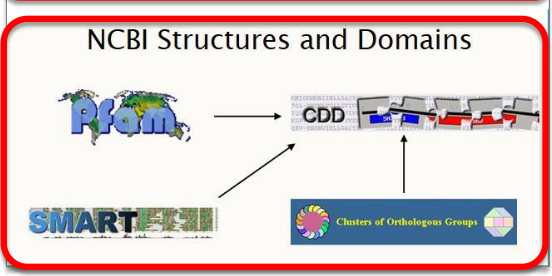
\includegraphics[width=.9\linewidth]{imgs/NCBI/2021-02-05_16-36-31_screenshot.png}
\end{center}
\end{itemize}




\subsection{GenBank}
\label{sec:orgc3befd7}
The GenBank sequence database is an open access, annotated collection of all publicly
available nucleotide sequences and their protein translations

\textbf{Submission}\\
\begin{itemize}
\item Only original sequences can be submitted to GenBank. Direct submissions are made to GenBank
via a Web-based form, or the stand-alone submission program, Sequin.
\item Upon receipt of a sequence submission, the GenBank staff examines the
originality of the data and assigns an accession number to the sequence and
performs quality assurance checks.
\item The submissions are then released to the public database, where the entries
are retrievable by Entrez or downloadable by FTP.
\end{itemize}


\subsubsection{GenBank Record Sample}
\label{sec:org2acabaa}
\textbf{Structure}
\begin{itemize}
\item Header
\item Features
\item Sequence
\end{itemize}


Most important \textbf{fields}:
\begin{itemize}
\item Accession code (eg. U49845): Stable, Reportable and Universal identifier
\item Version : tracks changes in sequence
\item CDS (Coding Sequence Region) : region of nucleotides that corresponds with the sequence of
amino acids in a protein (includes start and stop codons). This field include also the
respective translation protein. Annotation on the quality of the CDS can be
present.(experimental/not experimental)
\end{itemize}


\begin{verbatim}
LOCUS       SCU49845     5028 bp    DNA             PLN       21-JUN-1999
DEFINITION  Saccharomyces cerevisiae TCP1-beta gene, partial cds, and Axl2p
            (AXL2) and Rev7p (REV7) genes, complete cds.
ACCESSION   U49845
VERSION     U49845.1  GI:1293613
KEYWORDS    .
SOURCE      Saccharomyces cerevisiae (baker's yeast)
  ORGANISM  Saccharomyces cerevisiae
            Eukaryota; Fungi; Ascomycota; Saccharomycotina; Saccharomycetes;
            Saccharomycetales; Saccharomycetaceae; Saccharomyces.
REFERENCE   1  (bases 1 to 5028)
  AUTHORS   Torpey,L.E., Gibbs,P.E., Nelson,J. and Lawrence,C.W.
  TITLE     Cloning and sequence of REV7, a gene whose function is required for
            DNA damage-induced mutagenesis in Saccharomyces cerevisiae
  JOURNAL   Yeast 10 (11), 1503-1509 (1994)
  PUBMED    7871890
REFERENCE   2  (bases 1 to 5028)
  AUTHORS   Roemer,T., Madden,K., Chang,J. and Snyder,M.
  TITLE     Selection of axial growth sites in yeast requires Axl2p, a novel
            plasma membrane glycoprotein
  JOURNAL   Genes Dev. 10 (7), 777-793 (1996)
  PUBMED    8846915
REFERENCE   3  (bases 1 to 5028)
  AUTHORS   Roemer,T.
  TITLE     Direct Submission
  JOURNAL   Submitted (22-FEB-1996) Terry Roemer, Biology, Yale University, New
            Haven, CT, USA
FEATURES             Location/Qualifiers
     source          1..5028
                     /organism="Saccharomyces cerevisiae"
                     /db_xref="taxon:4932"
                     /chromosome="IX"
                     /map="9"
     CDS             <1..206
                     /codon_start=3
                     /product="TCP1-beta"
                     /protein_id="AAA98665.1"
                     /db_xref="GI:1293614"
                     /translation="SSIYNGISTSGLDLNNGTIADMRQLGIVESYKLKRAVVSSASEA
                     AEVLLRVDNIIRARPRTANRQHM"
     gene            687..3158
                     /gene="AXL2"
     CDS             687..3158
                     /gene="AXL2"
                     /note="plasma membrane glycoprotein"
                     /codon_start=1
                     /function="required for axial budding pattern of S.
                     cerevisiae"
                     /product="Axl2p"
                     /protein_id="AAA98666.1"
                     /db_xref="GI:1293615"
                     /translation="MTQLQISLLLTATISLLHLVVATPYEAYPIGKQYPPVARVNESF
                     TFQISNDTYKSSVDKTAQITYNCFDLPSWLSFDSSSRTFSGEPSSDLLSDANTTLYFN
                     VILEGTDSADSTSLNNTYQFVVTNRPSISLSSDFNLLALLKNYGYTNGKNALKLDPNE
                     VFNVTFDRSMFTNEESIVSYYGRSQLYNAPLPNWLFFDSGELKFTGTAPVINSAIAPE
                     TSYSFVIIATDIEGFSAVEVEFELVIGAHQLTTSIQNSLIINVTDTGNVSYDLPLNYV
                     YLDDDPISSDKLGSINLLDAPDWVALDNATISGSVPDELLGKNSNPANFSVSIYDTYG
                     DVIYFNFEVVSTTDLFAISSLPNINATRGEWFSYYFLPSQFTDYVNTNVSLEFTNSSQ
                     DHDWVKFQSSNLTLAGEVPKNFDKLSLGLKANQGSQSQELYFNIIGMDSKITHSNHSA
                     NATSTRSSHHSTSTSSYTSSTYTAKISSTSAAATSSAPAALPAANKTSSHNKKAVAIA
                     CGVAIPLGVILVALICFLIFWRRRRENPDDENLPHAISGPDLNNPANKPNQENATPLN
                     NPFDDDASSYDDTSIARRLAALNTLKLDNHSATESDISSVDEKRDSLSGMNTYNDQFQ
                     SQSKEELLAKPPVQPPESPFFDPQNRSSSVYMDSEPAVNKSWRYTGNLSPVSDIVRDS
                     YGSQKTVDTEKLFDLEAPEKEKRTSRDVTMSSLDPWNSNISPSPVRKSVTPSPYNVTK
                     HRNRHLQNIQDSQSGKNGITPTTMSTSSSDDFVPVKDGENFCWVHSMEPDRRPSKKRL
                     VDFSNKSNVNVGQVKDIHGRIPEML"
     gene            complement(3300..4037)
                     /gene="REV7"
     CDS             complement(3300..4037)
                     /gene="REV7"
                     /codon_start=1
                     /product="Rev7p"
                     /protein_id="AAA98667.1"
                     /db_xref="GI:1293616"
                     /translation="MNRWVEKWLRVYLKCYINLILFYRNVYPPQSFDYTTYQSFNLPQ
                     FVPINRHPALIDYIEELILDVLSKLTHVYRFSICIINKKNDLCIEKYVLDFSELQHVD
                     KDDQIITETEVFDEFRSSLNSLIMHLEKLPKVNDDTITFEAVINAIELELGHKLDRNR
                     RVDSLEEKAEIERDSNWVKCQEDENLPDNNGFQPPKIKLTSLVGSDVGPLIIHQFSEK
                     LISGDDKILNGVYSQYEEGESIFGSLF"
ORIGIN
        1 gatcctccat atacaacggt atctccacct caggtttaga tctcaacaac ggaaccattg
       61 ccgacatgag acagttaggt atcgtcgaga gttacaagct aaaacgagca gtagtcagct
      121 ctgcatctga agccgctgaa gttctactaa gggtggataa catcatccgt gcaagaccaa
      181 gaaccgccaa tagacaacat atgtaacata tttaggatat acctcgaaaa taataaaccg
      241 ccacactgtc attattataa ttagaaacag aacgcaaaaa ttatccacta tataattcaa
      301 agacgcgaaa aaaaaagaac aacgcgtcat agaacttttg gcaattcgcg tcacaaataa
      361 attttggcaa cttatgtttc ctcttcgagc agtactcgag ccctgtctca agaatgtaat
      421 aatacccatc gtaggtatgg ttaaagatag catctccaca acctcaaagc tccttgccga
      481 gagtcgccct cctttgtcga gtaattttca cttttcatat gagaacttat tttcttattc
      541 tttactctca catcctgtag tgattgacac tgcaacagcc accatcacta gaagaacaga
      601 acaattactt aatagaaaaa ttatatcttc ctcgaaacga tttcctgctt ccaacatcta
      661 cgtatatcaa gaagcattca cttaccatga cacagcttca gatttcatta ttgctgacag
      721 ctactatatc actactccat ctagtagtgg ccacgcccta tgaggcatat cctatcggaa
      781 aacaataccc cccagtggca agagtcaatg aatcgtttac atttcaaatt tccaatgata
      841 cctataaatc gtctgtagac aagacagctc aaataacata caattgcttc gacttaccga
      901 gctggctttc gtttgactct agttctagaa cgttctcagg tgaaccttct tctgacttac
      961 tatctgatgc gaacaccacg ttgtatttca atgtaatact cgagggtacg gactctgccg
     1021 acagcacgtc tttgaacaat acataccaat ttgttgttac aaaccgtcca tccatctcgc
     1081 tatcgtcaga tttcaatcta ttggcgttgt taaaaaacta tggttatact aacggcaaaa
     1141 acgctctgaa actagatcct aatgaagtct tcaacgtgac ttttgaccgt tcaatgttca
     1201 ctaacgaaga atccattgtg tcgtattacg gacgttctca gttgtataat gcgccgttac
     1261 ccaattggct gttcttcgat tctggcgagt tgaagtttac tgggacggca ccggtgataa
     1321 actcggcgat tgctccagaa acaagctaca gttttgtcat catcgctaca gacattgaag
     1381 gattttctgc cgttgaggta gaattcgaat tagtcatcgg ggctcaccag ttaactacct
     1441 ctattcaaaa tagtttgata atcaacgtta ctgacacagg taacgtttca tatgacttac
     1501 ctctaaacta tgtttatctc gatgacgatc ctatttcttc tgataaattg ggttctataa
     1561 acttattgga tgctccagac tgggtggcat tagataatgc taccatttcc gggtctgtcc
     1621 cagatgaatt actcggtaag aactccaatc ctgccaattt ttctgtgtcc atttatgata
     1681 cttatggtga tgtgatttat ttcaacttcg aagttgtctc cacaacggat ttgtttgcca
     1741 ttagttctct tcccaatatt aacgctacaa ggggtgaatg gttctcctac tattttttgc
     1801 cttctcagtt tacagactac gtgaatacaa acgtttcatt agagtttact aattcaagcc
     1861 aagaccatga ctgggtgaaa ttccaatcat ctaatttaac attagctgga gaagtgccca
     1921 agaatttcga caagctttca ttaggtttga aagcgaacca aggttcacaa tctcaagagc
     1981 tatattttaa catcattggc atggattcaa agataactca ctcaaaccac agtgcgaatg
     2041 caacgtccac aagaagttct caccactcca cctcaacaag ttcttacaca tcttctactt
     2101 acactgcaaa aatttcttct acctccgctg ctgctacttc ttctgctcca gcagcgctgc
     2161 cagcagccaa taaaacttca tctcacaata aaaaagcagt agcaattgcg tgcggtgttg
     2221 ctatcccatt aggcgttatc ctagtagctc tcatttgctt cctaatattc tggagacgca
     2281 gaagggaaaa tccagacgat gaaaacttac cgcatgctat tagtggacct gatttgaata
     2341 atcctgcaaa taaaccaaat caagaaaacg ctacaccttt gaacaacccc tttgatgatg
     2401 atgcttcctc gtacgatgat acttcaatag caagaagatt ggctgctttg aacactttga
     2461 aattggataa ccactctgcc actgaatctg atatttccag cgtggatgaa aagagagatt
     2521 ctctatcagg tatgaataca tacaatgatc agttccaatc ccaaagtaaa gaagaattat
     2581 tagcaaaacc cccagtacag cctccagaga gcccgttctt tgacccacag aataggtctt
     2641 cttctgtgta tatggatagt gaaccagcag taaataaatc ctggcgatat actggcaacc
     2701 tgtcaccagt ctctgatatt gtcagagaca gttacggatc acaaaaaact gttgatacag
     2761 aaaaactttt cgatttagaa gcaccagaga aggaaaaacg tacgtcaagg gatgtcacta
     2821 tgtcttcact ggacccttgg aacagcaata ttagcccttc tcccgtaaga aaatcagtaa
     2881 caccatcacc atataacgta acgaagcatc gtaaccgcca cttacaaaat attcaagact
     2941 ctcaaagcgg taaaaacgga atcactccca caacaatgtc aacttcatct tctgacgatt
     3001 ttgttccggt taaagatggt gaaaattttt gctgggtcca tagcatggaa ccagacagaa
     3061 gaccaagtaa gaaaaggtta gtagattttt caaataagag taatgtcaat gttggtcaag
     3121 ttaaggacat tcacggacgc atcccagaaa tgctgtgatt atacgcaacg atattttgct
     3181 taattttatt ttcctgtttt attttttatt agtggtttac agatacccta tattttattt
     3241 agtttttata cttagagaca tttaatttta attccattct tcaaatttca tttttgcact
     3301 taaaacaaag atccaaaaat gctctcgccc tcttcatatt gagaatacac tccattcaaa
     3361 attttgtcgt caccgctgat taatttttca ctaaactgat gaataatcaa aggccccacg
     3421 tcagaaccga ctaaagaagt gagttttatt ttaggaggtt gaaaaccatt attgtctggt
     3481 aaattttcat cttcttgaca tttaacccag tttgaatccc tttcaatttc tgctttttcc
     3541 tccaaactat cgaccctcct gtttctgtcc aacttatgtc ctagttccaa ttcgatcgca
     3601 ttaataactg cttcaaatgt tattgtgtca tcgttgactt taggtaattt ctccaaatgc
     3661 ataatcaaac tatttaagga agatcggaat tcgtcgaaca cttcagtttc cgtaatgatc
     3721 tgatcgtctt tatccacatg ttgtaattca ctaaaatcta aaacgtattt ttcaatgcat
     3781 aaatcgttct ttttattaat aatgcagatg gaaaatctgt aaacgtgcgt taatttagaa
     3841 agaacatcca gtataagttc ttctatatag tcaattaaag caggatgcct attaatggga
     3901 acgaactgcg gcaagttgaa tgactggtaa gtagtgtagt cgaatgactg aggtgggtat
     3961 acatttctat aaaataaaat caaattaatg tagcatttta agtataccct cagccacttc
     4021 tctacccatc tattcataaa gctgacgcaa cgattactat tttttttttc ttcttggatc
     4081 tcagtcgtcg caaaaacgta taccttcttt ttccgacctt ttttttagct ttctggaaaa
     4141 gtttatatta gttaaacagg gtctagtctt agtgtgaaag ctagtggttt cgattgactg
     4201 atattaagaa agtggaaatt aaattagtag tgtagacgta tatgcatatg tatttctcgc
     4261 ctgtttatgt ttctacgtac ttttgattta tagcaagggg aaaagaaata catactattt
     4321 tttggtaaag gtgaaagcat aatgtaaaag ctagaataaa atggacgaaa taaagagagg
     4381 cttagttcat cttttttcca aaaagcaccc aatgataata actaaaatga aaaggatttg
     4441 ccatctgtca gcaacatcag ttgtgtgagc aataataaaa tcatcacctc cgttgccttt
     4501 agcgcgtttg tcgtttgtat cttccgtaat tttagtctta tcaatgggaa tcataaattt
     4561 tccaatgaat tagcaatttc gtccaattct ttttgagctt cttcatattt gctttggaat
     4621 tcttcgcact tcttttccca ttcatctctt tcttcttcca aagcaacgat ccttctaccc
     4681 atttgctcag agttcaaatc ggcctctttc agtttatcca ttgcttcctt cagtttggct
     4741 tcactgtctt ctagctgttg ttctagatcc tggtttttct tggtgtagtt ctcattatta
     4801 gatctcaagt tattggagtc ttcagccaat tgctttgtat cagacaattg actctctaac
     4861 ttctccactt cactgtcgag ttgctcgttt ttagcggaca aagatttaat ctcgttttct
     4921 ttttcagtgt tagattgctc taattctttg agctgttctc tcagctcctc atatttttct
     4981 tgccatgact cagattctaa ttttaagcta ttcaatttct ctttgatc
//
\end{verbatim}



\subsubsection{Search field restrictions}
\label{sec:orgd9010d9}
We can add the following field restrictions keywords when we search in GenBank

\begin{itemize}
\item \textbf{[Title]} : Definition line glyceraldehyde 3
phosphate dehydrogenase[Title]
\item \textbf{[Organism]} : NCBI's taxonomy mouse[organism];
green plants[organism];
\item \textbf{[Properties]}: molecule type, location, database source
biomol\textsubscript{mrna}[properties]; biomol\textsubscript{genomic}[properties];
gene\textsubscript{in}\textsubscript{mitochondrion}[properties]; srcdb pdb[properties]
\item \textbf{[Filter]}: subsets of data, Entrez links
all[filter]; nucleotide mapview[filter]; nucleotide omim[filter]
\end{itemize}


\subsubsection{Division organization}
\label{sec:org34ddf38}
Records are divided into two types of \emph{divisions}

\textbf{12 Traditional Divisions}\\
\begin{itemize}
\item PRI Primate
\item PLN Plant and Fungal
\item BCT Bacterial and Archeal
\item INV Invertebrate
\item ROD Rodent
\item VRL Viral
\item VRT Other Vertebrate
\item MAM Mammalian
\item PHG Phage
\item SYN Synthetic (cloning vectors)
\item ENV Environmental Samples
\item UNA Unannotated
\end{itemize}

\uline{Features} :
\begin{itemize}
\item Direct Submissions
\item Accurate
\item Well characterized
\end{itemize}

\textbf{BULK Divisions}\\
\begin{itemize}
\item EST Expressed Sequence Tag
\item GSS Genome Survey Sequence
\item HTG High Throughput Genomic
\item STS Sequence Tagged Site
\item HTC High Throughput cDNA
\item PAT Patent
\end{itemize}

\uline{Features}:
\begin{itemize}
\item Batch Submission
\item Inaccurate
\item Poorly characterized
\end{itemize}


\subsection{RefSeq}
\label{sec:org8733820}
The Reference Sequence (RefSeq) database is an open access, annotated and curated
collection of publicly available nucleotide sequences (DNA, RNA) and their protein products.
This database is built by National Center for Biotechnology Information (NCBI), and, unlike
GenBank, \uline{provides only a single record for each natural biological molecule} (i.e. DNA, RNA or
protein) for major organisms ranging from viruses to bacteria to eukaryotes.

For each model organism, RefSeq aims to provide separate and linked records for the genomic
DNA, the gene transcripts, and the proteins arising from those transcripts. RefSeq is limited
to major organisms for which sufficient data are available (more than 66,000 distinct “named”
organisms as of September 2011), while GenBank includes sequences for any organism
submitted

\subsubsection{Difference RefSeq vs GenBank}
\label{sec:orgce64ade}


\begin{center}
\begin{tabular}{ll}
Genbank & RefSeq\\
\hline
Not Curated & Curated\\
Author submits & NCBI creates from genbank data\\
Multiple Records for same loci & Single records for each molecule of major organisms\\
No limit of species & Limited number of organisms\\
Akin to primary literature & Akin to review articles\\
 & \\
\end{tabular}
\end{center}

\begin{center}
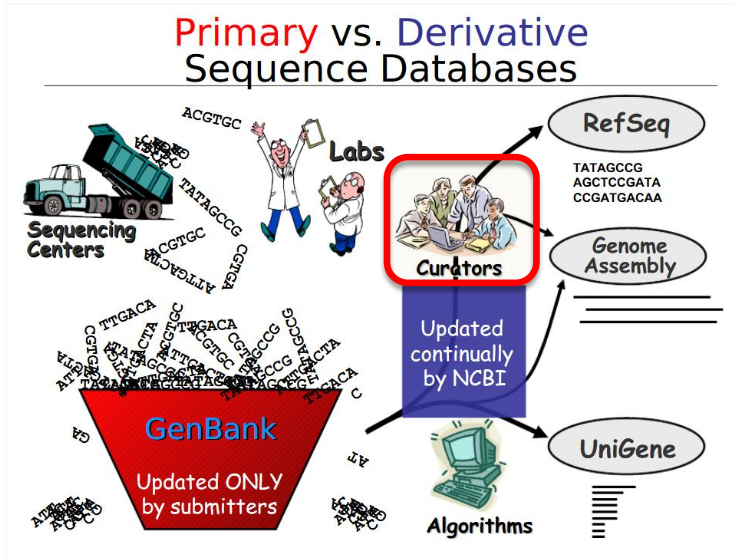
\includegraphics[width=.9\linewidth]{NCBI/sw_2020-12-15_17-15-34.png}
\end{center}


\subsubsection{RefSeq Categories}
\label{sec:orgf848860}
\begin{center}
\begin{tabular}{ll}
Category & Description\\
\hline
NC & Complete genomic molecules\\
NG & Incomplete genomic region\\
NM & mRNA\\
NR & ncRNA\\
NP & Protein\\
XM & predicted mRNA model\\
XR & predicted ncRNA model\\
XP & predicted Protein model (eukaryotic sequences)\\
WP & predicted Protein model (prokaryotic sequences)\\
\end{tabular}
\end{center}


\subsubsection{RefSeq Status}
\label{sec:orgcdff28f}
\begin{itemize}
\item Model : No individual review
\item Inferred : Predicted by genome sequence analysis
\item Predicted : No individual review, some aspect predicted
\item Reviewed : Reviewed by NCBI staff
\item Validated : No final review, initial review performed
\end{itemize}

\subsection{Gene}
\label{sec:org9df367d}
Gene supplies gene-specific connections in the nexus of map, sequence,
expression, structure, function, citation, and homology data.

Unique identifiers are assigned to genes with defining sequences, genes with
known map positions, and genes inferred from phenotypic information. These gene
identifiers are used throughout NCBI's databases and tracked through updates of
annotation.

\subsubsection{NCBI Record}
\label{sec:org91ccbf7}
A NCBI Gene record may include:
\begin{itemize}
\item nomenclature,
\item Reference Sequences (RefSeqs),
\item maps,
\item pathways,
\item variations,
\item phenotypes,
\item links to genome-, phenotype-, and locus-specific resources worldwide
\end{itemize}

\subsubsection{NCBI Gene Query}
\label{sec:orgc77131c}

\begin{center}
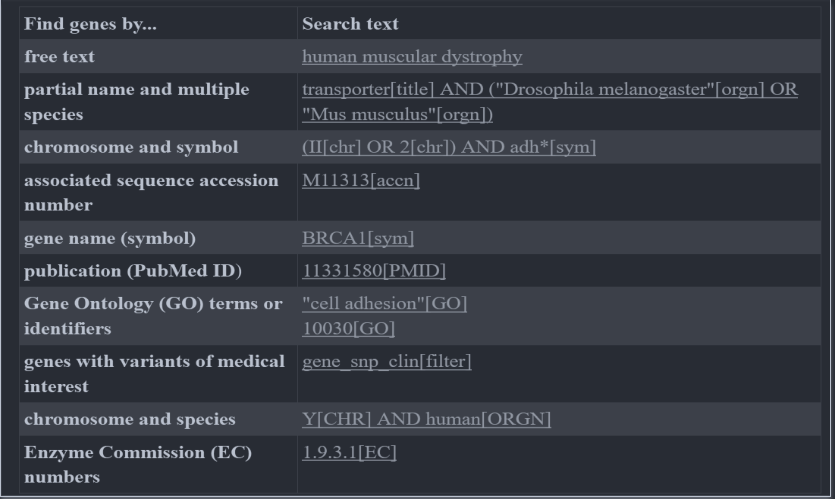
\includegraphics[width=.9\linewidth]{imgs/NCBI/2021-02-05_17-36-33_screenshot.png}
\end{center}


\subsection{OMIM (Online Mendelian Inheritance in Man)}
\label{sec:orge4e5dc3}
The full-text overviews in OMIM contain information on all known
mendelian disorders and over 16,000 genes. It is updated daily.
\begin{itemize}
\item OMIM focuses on the relationship between phenotype and genotype.
\item This database was initiated in the early 1960s by Dr. Victor A. McKusick as a
catalog of mendelian traits and disorders (Mendelian Inheritance in Man –
MIM). The online version, OMIM, was created in 1985 by a collaboration between
the NLM and the Johns Hopkins University.
\end{itemize}


\subsection{dbSNP}
\label{sec:org9fa005a}
The database contains actually a range of molecular variations:
\begin{enumerate}
\item SNPs
\item short deletion and insertion polymorphisms (indels/DIPs)
\item microsatellite markers or Short Tandem Repeats (STRs)
\item multinucleotide polymorphisms (MNPs)
\end{enumerate}


\textbf{Dataflow}\\

\begin{center}
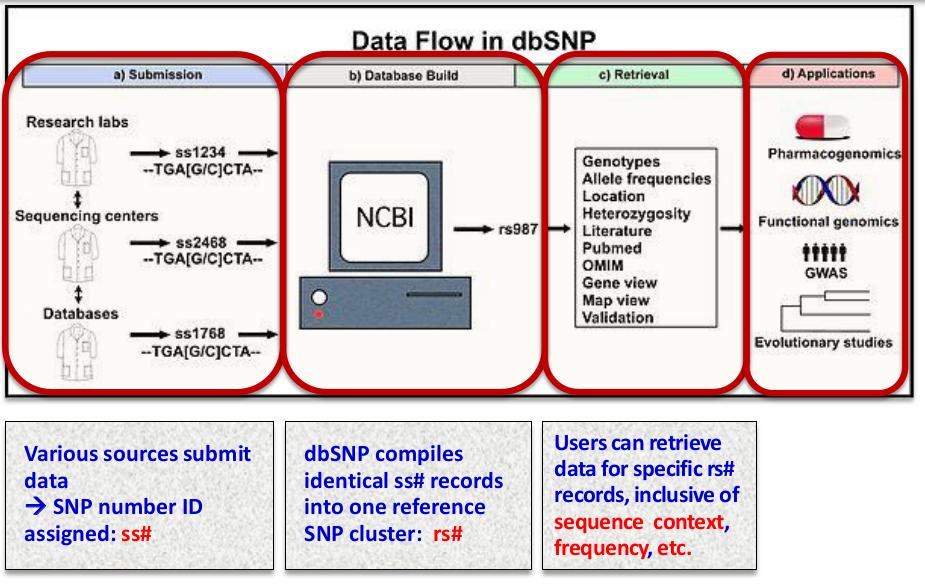
\includegraphics[width=.9\linewidth]{imgs/NCBI/2021-02-05_17-45-37_screenshot.png}
\end{center}


\subsubsection{GWAS}
\label{sec:orgc33b0eb}
Sequence variations might be responsible for individual phenotypic characteristics,
including a person's propensity toward complex disorders such as heart disease and cancer.


\begin{center}
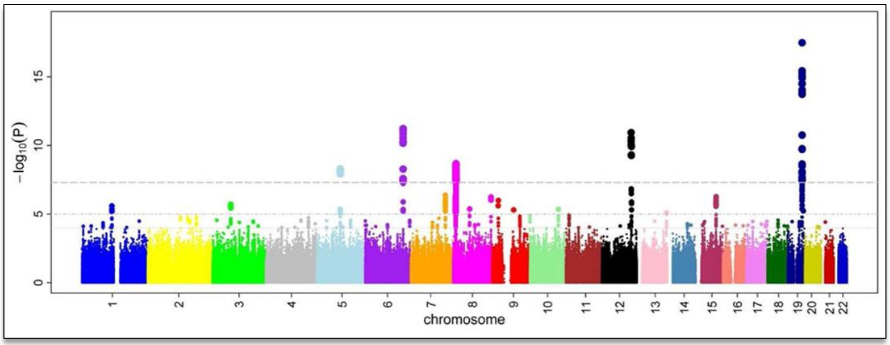
\includegraphics[width=.9\linewidth]{imgs/NCBI/2021-02-05_17-46-17_screenshot.png}
\end{center}

A Manhattan plot depicting several strongly associated risk loci. Each dot
represents a SNP, X-axis: genomic location, Y-axis: association level.

A GWA study investigating microcirculation, the tops indicates genetic variants that
more often are found in individuals with constrictions in small blood vessels.

\subsection{Nucleotide}
\label{sec:org22c52aa}
The Nucleotide database is a collection of sequences from several sources,
including GenBank, RefSeq, TPA and PDB. Genome, gene and transcript sequence
data provide the foundation for biomedical research and discovery.


\subsection{Exercises}
\label{sec:org074396d}
\subsubsection{Exercise 1}
\label{sec:org2d14835}
\begin{itemize}
\item \textbf{Question}\\
\end{itemize}
In NCBI ``Nucleotide'', find all entries

containing:                  mRNA sequences

coding for:                   chymotrypsin and trypsin  (use the field: ``Protein name'')

from:                             all organisms except Plant, Fungal, and Viral

which have been:         reviewed or validated in RefSeq.

(Notice that in NCBI searches the boolean have to be uppercase :

``AND'', ``OR'' , ``NOT'')




How many entries have you found ?


\begin{itemize}
\item \textbf{Answer}\\

\begin{verbatim}
  "biomol mrna"[Properties] AND ("trypsin"[Protein Name] OR "chymotrypsin"[Protein Name]) NOT ("gbdiv pln"[Properties] OR "gbdiv vrl"[Properties]) AND ("srcdb refseq reviewed"[Properties] OR "srcdb refseq validated"[Properties])
\end{verbatim}
\end{itemize}

\subsubsection{Exercise 2}
\label{sec:orgd3331c6}
\begin{itemize}
\item \textbf{Question}\\
In the Gene database, look for the gene coding for the NP\textsubscript{073728} protein.

\begin{enumerate}
\item Which is its cytogenetic location ?

\item In which biological process is the protein involved, according to the GO classification, TAS code ?

\item What is the RefSeq Accession Number of the mRNA molecule coding for it?  Is it a reviewed entry?
\end{enumerate}
\end{itemize}


\begin{itemize}
\item \textbf{Answer}\\

\begin{enumerate}
\item Location: 2q37.3
\item circadian rhythm       GO:0007623
\item NM\textsubscript{022817.3} Reviewed
\end{enumerate}
\end{itemize}
\subsubsection{Exercise 3}
\label{sec:org11cfcda}
\begin{itemize}
\item \textbf{Question}
\begin{enumerate}
\item How many genes in the «Gene» database have as source the species Homo sapiens ?
\item How many of them are «protein coding» ?
\item How many are «pseudo-genes» ?
\item How many are «non-coding RNA» ?
\end{enumerate}

\item \textbf{Answer}
\begin{enumerate}
\item 61745 - ``human''[Organism]
\item 19786 - (``human''[Organism]) AND ``genetype protein coding''[Properties]
\item 16552 - (``human''[Organism]) AND ``genetype pseudo''[Properties]
\item 17455 - (``genetype ncrna''[Properties]) AND ``human''[Organism]
\end{enumerate}
\end{itemize}
\section{Experimental Methods}
\label{sec:org1f6900b}
\subsection{X-ray Crystallography}
\label{sec:orgc070c0f}
\emph{X-ray crystallography} (XRC) is the experimental science determining the atomic and molecular
structure of a crystal, in which the crystalline structure causes a beam of incident X-rays to
diffract into many specific directions. By measuring the angles and intensities of these
diffracted beams, a crystallographer can produce a three-dimensional picture of the density of
electrons within the crystal. From this electron density, the mean positions of the atoms in
the crystal can be determined, as well as their chemical bonds, their crystallographic
disorder, and various other information.

\#+Xray Cristallography to structure scheme 
\begin{center}
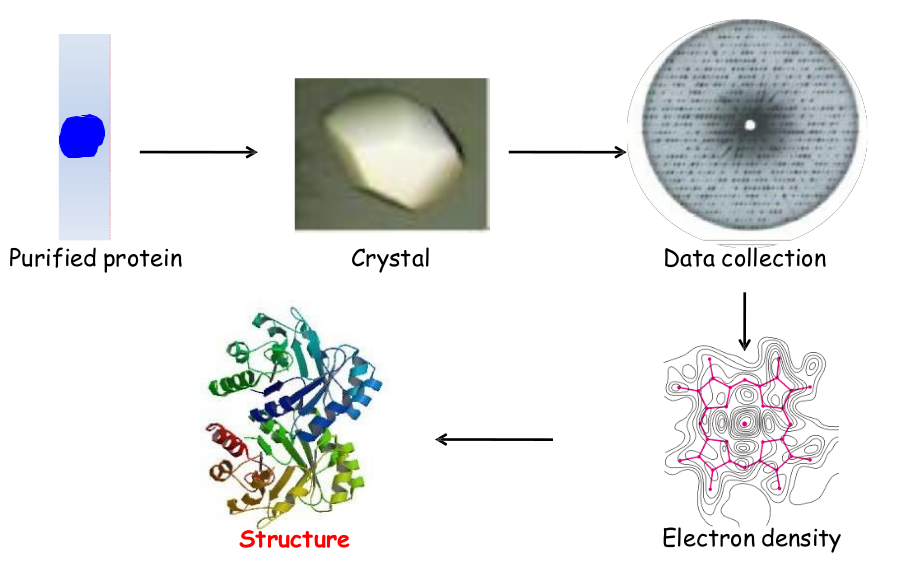
\includegraphics[width=.9\linewidth]{PDB/crystellographyschemefull_2020-12-03_17-02-06.png}
\end{center}


\begin{enumerate}
\item \textbf{Crystals Formation} : A crystal is a three-dimensional regular structure formed by many
identical molecules. Proteins are large objects with irregular shapes and it is impossible
to pack them into a crystal without forming large holes or channels between the individual
molecules.

The formation of a crystal strongly depends on a number of different parameters, such as
pH, temperature, protein concentration. Well ordered protein crystals diffract X-rays.

The atoms in a crystal are not static, but oscillate about their mean positions, usually by
less than a few tenths of an angstrom. X-ray crystallography allows measuring the size of
these oscillations.

Due to the ordered molecular packing, the crystal behaves as a very powerful amplifier

\item \textbf{Why X-rays} : In order to measure something accurately you need the appropriate ruler. The
X-rays wavelength[10 Å and 0.01 Å] has the same order of magnitude of a covalent bond. The
type of X-rays used by crystallographers are \textasciitilde{} 0.5 to 1.5 Å long.
\end{enumerate}


\subsection{NMR Spectroscopy}
\label{sec:orgb944622}
\textbf{Nuclear magnetic resonance spectroscopy}, most commonly known as NMR spectroscopy or magnetic
resonance spectroscopy (MRS), is a spectroscopic technique to observe local magnetic fields
around atomic nuclei. 

\begin{itemize}
\item The sample is placed in a magnetic field and the NMR signal is produced by excitation of the
nuclei sample with \emph{radio waves} into \emph{nuclear magnetic resonance}, which is detected with
sensitive radio receivers.
\item The intramolecular magnetic field around an atom in a molecule changes the resonance
frequency, thus giving access to details of the electronic structure of a molecule and its
individual functional groups.

\item A distinctive set of observed resonances may be analyzed to give a list of atomic nuclei
that are close to one another, and to characterize the local conformation of atoms that are
bonded together. This list of restraints is then used to build models of the protein that
shows the location of each atom. The technique is currently limited to small or medium
proteins, since large proteins present problems with overlapping peaks in the NMR spectra.
\end{itemize}


\textbf{Variation among models}\\
\begin{itemize}
\item can represent actual flexibility and thermal motion
\item can mean uncertainty in the atomic positions
\end{itemize}

To distinguish between the two, specific NMR experiments can be used to measure the dynamics
of individual atoms.

\subsubsection{Pros and Cons}
\label{sec:orgeb3c9e8}
\textbf{Difficulties}
\begin{itemize}
\item protein in solution: protein has to be soluble
\item insensitive method: requires high concentrations of proteins
\item direct determination of 3D structures for small proteins only
(up to 50-60 kD)
\end{itemize}


\textbf{Advantages}
\begin{itemize}
\item protein in solution: no crystal packing artefacts, allows direct
\end{itemize}
binding experiments, hydrodynamic and folding studies
\begin{itemize}
\item assignment of mobile regions (loops) possible: no gaps in
\end{itemize}
structure


\subsection{Cry-electron microscopy}
\label{sec:orgdaa4032}
Electron microscopy, frequently referred to as 3DEM, is also used to determine 3D structures
of large macromolecular assemblies. A beam of electrons and a system of electron lenses is
used to image the biomolecule directly. Several tricks are required to obtain a 3D structure
from 2D projection images produced by transmission electron microscopes. The most commonly
used technique today involves imaging of many thousands of different single particles
preserved in a thin layer of non-crystalline ice (cryo-EM). Provided these views show the
molecule in myriad different orientations, a computational approach akin to that used for
computerized axial tomography or CAT scans in medicine will yield a 3D mass density map. With
a sufficient number of single particles, the 3DEM maps can then be interpreted by fitting an
atomic model of the macromolecule into the map, just as macromolecular crystallographers
interpret their electron density maps.



\section{Database}
\label{sec:org224ecf3}
A database is an organized collection of data, generally stored and accessed electronically from a computer system.
\end{document}
